\chapter{Uncertainty and Controls}\label{ch:controls}

\begin{chapterintro}
Suppose you time ten swings of a pendulum and get $14.2$~s, and a friend timing the same pendulum gets $14.5$~s. Did the pendulum change, or did the two of you press the stopwatch at slightly different moments? You cannot answer until each number carries an error bar. First-year laboratories teach this lesson for measurements made with rulers and clocks (see \cite{hrw}). This chapter teaches it for the numbers produced by a computational study: an rms error on a set of held-out zeros, a correlation between a prediction and the truth, an in-sample fit quality.

We address three questions. First, \emph{how uncertain is a score computed from a finite set of data?} The tools are the standard error, the bootstrap, and its block version for data whose neighbors are correlated. Second, \emph{when a model fits its training data well, did it find structure or can it fit anything?} The tools are permutation tests, surrogate data (shuffled, phase-randomized, amplitude-adjusted) and the general idea of positive and negative controls. Third, \emph{which analyses were planned before the data were seen?} Here we distinguish confirmatory from exploratory analysis and explain why a statistic invented after looking at the data cannot carry a significance claim.

Where this shows up in the paper \cite{soniR1}: every bracketed interval in Secs.~III and IV and in Tables~II, IV and V is a bootstrap percentile interval; the block-bootstrap check in Sec.~III uses block lengths 3 to 20; the ``Permutation and surrogate tests'' paragraph of Sec.~III refits the operator to shuffled and phase-randomized targets; Appendix~A steps 12, 13, 18, 22 and 23 record exactly how; and Sec.~IV qualifies its frequency-alignment check with the words ``the statistic was defined after the data were seen, so the check is exploratory''. After this chapter you will know what each of those sentences means and why it is there.
\end{chapterintro}

\begin{prerequisites}
\item Chapter~\ref{ch:probability}: random variables, mean, variance, standard deviation, rms, covariance, Pearson correlation, autocorrelation of a sequence, standard error, the idea of a confidence interval, the law of large numbers, random number generators and seeds, the exponential distribution of gaps in a Poisson process.
\item Chapter~\ref{ch:fourier-transform}: the discrete Fourier transform (DFT) and the FFT, power spectrum, the Wiener--Khinchin connection between autocorrelation and power spectrum, and the basic idea of phase randomization.
\item Chapter~\ref{ch:generalization}: training and held-out sets, in-sample and out-of-sample error, the null model, saturated models, serial correlation of the zero fluctuations, simple kriging.
\item Chapter~\ref{ch:series}: the geometric series and its sum.
\item First-year physics: measurement uncertainty as an idea, averaging repeated measurements.
\end{prerequisites}

%======================================================================
\section{Sampling variability: every score is one draw}\label{sec:controls-variability}

Imagine scoring a model on zeros 401--500 and getting rms error $0.369$ (in units of the local mean spacing; recall from Chapter~\ref{ch:generalization} that the rms error is $\sqrt{\frac1n\sum_j(\text{pred}_j-\text{true}_j)^2}$). Had you scored on a different hundred zeros from the same height range, you would have gotten a somewhat different number. The score depends on \emph{which} levels happened to be in the test set. This dependence is called \textbf{sampling variability}, and the first task of this chapter is to measure it.

\subsection{Estimators and their sampling distributions}

We model the data $x_1,\dots,x_n$ as the observed values of random variables $X_1,\dots,X_n$. In the simplest model the $X_j$ are \textbf{independent and identically distributed} (iid): each is drawn from the same distribution, with mean $\mu$ and variance $\sigma^2$, and knowing one tells you nothing about another.

A \textbf{statistic} (or \textbf{estimator}) is any number computed from the data, written $\hat\theta=\hat\theta(x_1,\dots,x_n)$. The sample mean $\bar x=\frac1n\sum_j x_j$ is one; so are the rms error and the correlation of a prediction with the truth. Because the data are random, so is $\hat\theta$. Its probability distribution over repeated experiments is the \textbf{sampling distribution}, and the standard deviation of the sampling distribution is the \textbf{standard error} (SE) of $\hat\theta$.

\subsection{The standard error of a mean}

For the mean of iid data we can compute the standard error exactly. Write $\bar X=\frac1n\sum_{j=1}^n X_j$. Its expected value is
\begin{equation}
E[\bar X]=\frac1n\sum_{j=1}^n E[X_j]=\frac1n\cdot n\mu=\mu .
\label{eq:controls-meanmean}
\end{equation}
For the variance, start from the definition $\mathrm{Var}(\bar X)=E[(\bar X-\mu)^2]$ and write $\bar X-\mu=\frac1n\sum_j(X_j-\mu)$:
\begin{align}
\mathrm{Var}(\bar X)&=E\Big[\Big(\frac1n\sum_{i=1}^n(X_i-\mu)\Big)\Big(\frac1n\sum_{j=1}^n(X_j-\mu)\Big)\Big]\nonumber\\
&=\frac1{n^2}\sum_{i=1}^n\sum_{j=1}^n E[(X_i-\mu)(X_j-\mu)]\quad\text{(expand, expectation is linear)}\nonumber\\
&=\frac1{n^2}\sum_{i=1}^n\sum_{j=1}^n \mathrm{Cov}(X_i,X_j)\quad\text{(definition of covariance, Ch.~\ref{ch:probability})}\nonumber\\
&=\frac1{n^2}\sum_{i=1}^n \sigma^2\quad\text{(independence: $\mathrm{Cov}=0$ for $i\ne j$; $\mathrm{Cov}(X_i,X_i)=\sigma^2$)}\nonumber\\
&=\frac{\sigma^2}{n}.
\label{eq:controls-varmean}
\end{align}
So the standard error of the mean is $\sigma/\sqrt n$. Quadrupling the data halves the error bar; this is the familiar rule from averaging repeated measurements.

We do not know $\sigma$, so we estimate it from the data. Two estimates are in common use:
\begin{equation}
\hat\sigma^2=\frac1n\sum_{j=1}^n(x_j-\bar x)^2\quad\text{(plug-in)},\qquad
s^2=\frac1{n-1}\sum_{j=1}^n(x_j-\bar x)^2\quad\text{(sample variance)}.
\label{eq:controls-twovar}
\end{equation}
Chapter~\ref{ch:probability} explained that $s^2$ is unbiased ($E[s^2]=\sigma^2$) while $\hat\sigma^2=\frac{n-1}{n}s^2$ is slightly too small on average. The estimated standard error of the mean is
\begin{equation}
\widehat{\mathrm{SE}}(\bar x)=\frac{s}{\sqrt n}.
\label{eq:controls-se}
\end{equation}

\begin{sample}{Standard error of a small sample}
Five measurements are $x=(3,7,4,9,2)$. Find $\bar x$, $s$, $\widehat{\mathrm{SE}}(\bar x)$ and the plug-in variance $\hat\sigma^2$.

\textbf{Step 1:} Mean. $\bar x=(3+7+4+9+2)/5=25/5=5$.

\textbf{Step 2:} Deviations $x_j-\bar x$: $-2,\,2,\,-1,\,4,\,-3$. Squares: $4,4,1,16,9$, sum $34$.

\textbf{Step 3:} $s^2=34/4=8.5$, so $s=\sqrt{8.5}=2.9155$.

\textbf{Step 4:} $\widehat{\mathrm{SE}}=s/\sqrt5=2.9155/2.2361=1.3038$.

\textbf{Step 5:} $\hat\sigma^2=34/5=6.8$.

\[
\boxed{\bar x=5,\quad s=2.916,\quad \widehat{\mathrm{SE}}(\bar x)=1.304,\quad \hat\sigma^2=6.8}
\]
\end{sample}

\subsection{Why we need something more general}

Equation~\eqref{eq:controls-se} is special to the mean. The scores in the paper are an rms error, $\sqrt{\frac1n\sum_j r_j^2}$, and a Pearson correlation, $\corr(a,b)=\sum_j(a_j-\bar a)(b_j-\bar b)/\sqrt{\sum_j(a_j-\bar a)^2\sum_j(b_j-\bar b)^2}$. Neither has a simple exact standard-error formula, and the approximate formulas found in statistics books assume Gaussian data. We want a method that works for \emph{any} statistic you can compute. That method is the bootstrap.

\begin{checkpoint}
A held-out set is enlarged from 100 to 400 levels drawn from the same height range. If the levels were independent, by roughly what factor would the standard error of the held-out mean fluctuation shrink?
\end{checkpoint}
\checkanswer{By $\sqrt{400/100}=2$, from Eq.~\eqref{eq:controls-varmean}: the SE scales as $1/\sqrt n$.}

\begin{keyideas}
\item Any number computed from data is a random draw from its sampling distribution; its standard deviation is the standard error.
\item For iid data, $\mathrm{Var}(\bar X)=\sigma^2/n$ (Eq.~\eqref{eq:controls-varmean}); estimate $\sigma$ by $s$.
\item rms errors and correlations need a more general method.
\end{keyideas}

%======================================================================
\section{The bootstrap}\label{sec:controls-bootstrap}

\subsection{The plug-in idea}

If we knew the distribution $F$ from which the data were drawn, we could estimate the standard error of any statistic by simulation: draw a fresh data set of size $n$ from $F$, compute $\hat\theta$, repeat thousands of times, and take the standard deviation. We do not know $F$. The \textbf{bootstrap} (Efron, 1979; see \cite{efron}) replaces $F$ by its best data-based estimate, the \textbf{empirical distribution} $\hat F$, which puts probability $1/n$ on each observed value $x_1,\dots,x_n$.

Drawing $n$ values from $\hat F$ means: choose one of the $n$ data points uniformly at random, write it down, put it back, and repeat $n$ times. This is \textbf{resampling with replacement}. The result $x^*=(x^*_1,\dots,x^*_n)$ is a \textbf{bootstrap resample}; some original points appear twice or more, some not at all. Computing the statistic on it gives a \textbf{bootstrap replicate} $\hat\theta^*$.

The bootstrap principle is the assumption that
\begin{equation}
\text{the distribution of }\hat\theta^*\text{ around }\hat\theta\quad\approx\quad\text{the distribution of }\hat\theta\text{ around the true }\theta.
\label{eq:controls-principle}
\end{equation}
A physical analogy: you cannot rerun the universe to get another set of zeros of the same height, so you treat the hundred zeros you have as a miniature population and rerun the sampling experiment inside it.

\subsection{The ideal bootstrap for the mean}

There are $n^n$ ordered resamples, all equally likely. The \textbf{ideal bootstrap} averages over all of them exactly. For the mean we can do this in closed form.

A single resampled value $X^*$ equals $x_j$ with probability $1/n$ for each $j$. Hence
\begin{align}
E^*[X^*]&=\sum_{j=1}^n\frac1n x_j=\bar x,\label{eq:controls-bootmean}\\
\mathrm{Var}^*(X^*)&=\sum_{j=1}^n\frac1n(x_j-\bar x)^2=\hat\sigma^2,\label{eq:controls-bootvar1}
\end{align}
where the star means ``in the bootstrap world'', with the data held fixed. The $n$ resampled values are drawn independently of each other, so Eq.~\eqref{eq:controls-varmean} applies inside the bootstrap world with $\sigma^2$ replaced by $\hat\sigma^2$:
\begin{equation}
\mathrm{Var}^*(\bar x^*)=\frac{\hat\sigma^2}{n}=\frac{n-1}{n}\cdot\frac{s^2}{n}\quad\text{(using $\hat\sigma^2=\tfrac{n-1}{n}s^2$, Eq.~\eqref{eq:controls-twovar})}.
\label{eq:controls-bootvarmean}
\end{equation}
The bootstrap standard error of the mean is therefore $\sqrt{(n-1)/n}$ times the usual one. For $n=100$ the factor is $0.995$; for $n=5$ it is $0.894$. The bootstrap is slightly optimistic for tiny samples, a first hint that it is a large-sample method.

\begin{sample}{The ideal bootstrap by enumeration}
Data $x=(1,2,6)$. List the bootstrap distribution of the mean exactly, and check its variance against Eq.~\eqref{eq:controls-bootvarmean}.

\textbf{Step 1:} A resample is fixed by how many times each value appears: counts $(k_1,k_2,k_6)$ with $k_1+k_2+k_6=3$. The number of ordered resamples with those counts is the multinomial coefficient $3!/(k_1!\,k_2!\,k_6!)$; the total over all count patterns is $3^3=27$.

\textbf{Step 2:} The sum of a resample is $k_1+2k_2+6k_6$, and the mean is the sum divided by 3. Tabulating all ten count patterns gives Table~\ref{tab:controls-enum}.

\textbf{Step 3:} Expected mean. Multiply each resample sum by its weight and add: $3\cdot1+4\cdot3+5\cdot3+6\cdot1+8\cdot3+9\cdot6+10\cdot3+13\cdot3+14\cdot3+18\cdot1=243$. Divide by the 27 resamples, and by 3 to turn sums into means: $243/(27\times3)=3$. This equals $\bar x=3$, as Eq.~\eqref{eq:controls-bootmean} requires.

\textbf{Step 4:} Expected squared mean: $\frac1{27}\sum(\text{weight}\times\text{mean}^2)=285/27=10.556$. So $\mathrm{Var}^*=10.556-3^2=1.556$.

\textbf{Step 5:} Formula: deviations from $\bar x=3$ are $-2,-1,3$, squares sum to $14$, so $\hat\sigma^2=14/3$ and $\hat\sigma^2/n=14/9=1.556$. They agree.

\[
\boxed{\mathrm{Var}^*(\bar x^*)=14/9=1.556,\qquad \mathrm{SE}_{\rm boot}=1.247}
\]
\end{sample}

\begin{table}[htbp]\centering
\caption{The complete bootstrap distribution of the mean for the data $(1,2,6)$. ``Weight'' is the number of the 27 equally likely ordered resamples with the given counts; the last column is the cumulative probability $F^*$.}\label{tab:controls-enum}
\begin{tabular}{cccccc}
\toprule
counts $(k_1,k_2,k_6)$ & example & sum & mean & weight & $F^*(\text{mean})$\\
\midrule
$(3,0,0)$ & $1,1,1$ & 3 & $1$ & 1 & $1/27$\\
$(2,1,0)$ & $1,1,2$ & 4 & $4/3$ & 3 & $4/27$\\
$(1,2,0)$ & $1,2,2$ & 5 & $5/3$ & 3 & $7/27$\\
$(0,3,0)$ & $2,2,2$ & 6 & $2$ & 1 & $8/27$\\
$(2,0,1)$ & $1,1,6$ & 8 & $8/3$ & 3 & $11/27$\\
$(1,1,1)$ & $1,2,6$ & 9 & $3$ & 6 & $17/27$\\
$(0,2,1)$ & $2,2,6$ & 10 & $10/3$ & 3 & $20/27$\\
$(1,0,2)$ & $1,6,6$ & 13 & $13/3$ & 3 & $23/27$\\
$(0,1,2)$ & $2,6,6$ & 14 & $14/3$ & 3 & $26/27$\\
$(0,0,3)$ & $6,6,6$ & 18 & $6$ & 1 & $27/27$\\
\bottomrule
\end{tabular}
\end{table}

\subsection{How many resamples are there?}

The table has ten rows because ten count patterns exist. In general, a count pattern is a list of $n$ non-negative integers summing to $n$. Picture $n$ stars (the draws) separated by $n-1$ bars into $n$ bins (the data points). Every arrangement of $2n-1$ symbols, $n$ of them stars, gives one pattern and vice versa, so the number of distinct resamples is
\begin{equation}
\binom{2n-1}{n}.
\label{eq:controls-distinct}
\end{equation}
For $n=3$ this is $\binom53=10$, matching the table. For $n=100$ held-out zeros it is $\binom{199}{100}\approx4.5\times10^{58}$. Enumeration is hopeless, so in practice we use the Monte Carlo bootstrap.

\subsection{The Monte Carlo bootstrap}

Draw $B$ resamples at random (with a seeded generator, so the result is reproducible; Chapter~\ref{ch:probability}), compute $\hat\theta^*_1,\dots,\hat\theta^*_B$, and use their standard deviation as the standard error. The Monte Carlo step adds its own small error. How large is that error? We quote one standard statistical result without proof (see \cite{efron}). For $B$ independent Gaussian draws with standard deviation $\sigma$, the sample variance $s_B^2$ has variance $2\sigma^4/(B-1)$. Its relative standard deviation is therefore $\sqrt{2/(B-1)}$. The standard deviation is $s_B=\sqrt{s_B^2}$, and a small relative change $\epsilon$ in $s_B^2$ produces a relative change of about $\epsilon/2$ in $s_B$, because $\sqrt{1+\epsilon}\approx1+\epsilon/2$ to first order in Taylor's expansion. So the relative error of $s_B$ is about $\tfrac12\sqrt{2/(B-1)}\approx1/\sqrt{2B}$. This is a heuristic: it holds when the bootstrap distribution is close to Gaussian. For $B=2\times10^4$ it gives $0.5\%$, which is negligible next to the sampling uncertainty itself.

\begin{pycode}
import numpy as np
rng = np.random.default_rng(0)          # seeded: reproducible
x = np.array([3., 7., 4., 9., 2.])
B = 20000
idx = rng.integers(0, len(x), size=(B, len(x)))  # B resamples of positions
means = x[idx].mean(axis=1)             # one bootstrap mean per row
print(means.std())                      # close to the exact 1.166
print(np.percentile(means, [2.5, 97.5]))  # percentile interval (see below)
\end{pycode}

For the five data of the first Sample Problem, Eq.~\eqref{eq:controls-bootvarmean} gives the exact ideal-bootstrap standard error $\sqrt{6.8/5}=\sqrt{1.36}=1.166$, and the listing reproduces it to within about one percent.

\subsection{Percentile intervals}

A standard error summarizes spread by one number. Often we want an interval. The \textbf{percentile interval} at level $1-\alpha$ (for example $95\%$, $\alpha=0.05$) takes the $\alpha/2$ and $1-\alpha/2$ quantiles of the bootstrap distribution. With the cumulative bootstrap distribution $F^*(v)=P^*(\hat\theta^*\le v)$, the $q$-quantile is the smallest value $v$ with $F^*(v)\ge q$. With $B$ sorted Monte Carlo replicates, it is (up to small interpolation conventions, such as the one \texttt{np.percentile} uses) the replicate at position $\lceil qB\rceil$; for $B=2\times10^4$ the $2.5\%$ point is the 500th sorted value and the $97.5\%$ point the 19\,500th.

\begin{sample}{Percentile intervals from the enumeration}
Using Table~\ref{tab:controls-enum}, find the $80\%$ and $95\%$ percentile intervals for the mean of $(1,2,6)$.

\textbf{Step 1:} $80\%$ interval: quantiles $0.10$ and $0.90$. The smallest mean with $F^*\ge0.10$: $F^*(1)=1/27=0.037$, $F^*(4/3)=4/27=0.148$. So the lower end is $4/3$.

\textbf{Step 2:} Upper end: $F^*(13/3)=23/27=0.852<0.90$, $F^*(14/3)=26/27=0.963\ge0.90$. So the upper end is $14/3$.

\textbf{Step 3:} $95\%$ interval: quantiles $0.025$ and $0.975$. $F^*(1)=0.037\ge0.025$ gives lower end $1$; $F^*(14/3)=0.963<0.975$ and $F^*(6)=1$ give upper end $6$.

\[
\boxed{80\%:\ [4/3,\ 14/3],\qquad 95\%:\ [1,\ 6]}
\]
The $95\%$ interval is the whole range of possible means: with $n=3$ the bootstrap has nothing to say at that level. Figure~\ref{fig:controls-bootstrap_enum} shows the distribution.
\end{sample}

\begin{figure}[htbp]\centering
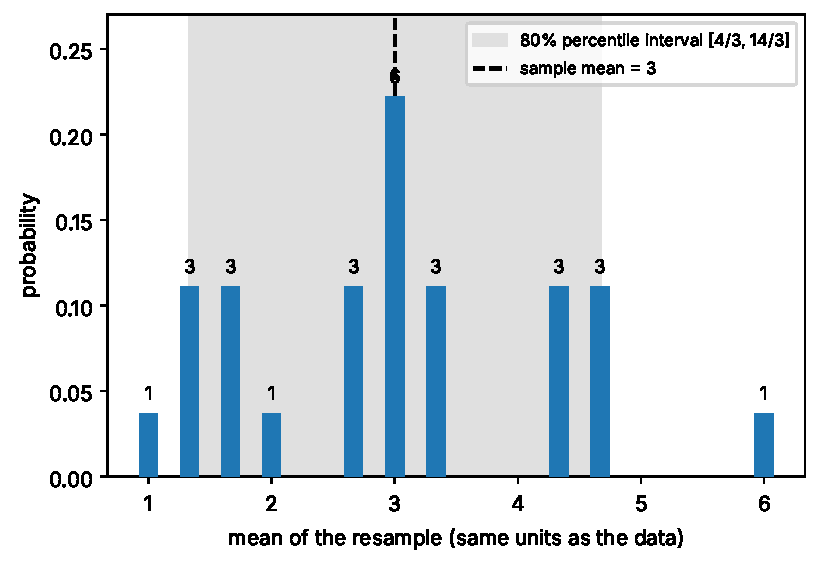
\includegraphics[width=0.85\linewidth]{figs/controls_bootstrap_enum.pdf}
\caption{The exact bootstrap distribution of the mean of the three data $(1,2,6)$, from Table~\ref{tab:controls-enum}. Bar labels give the number of the 27 ordered resamples producing each mean. The dashed line is the sample mean $3$; the shaded band is the $80\%$ percentile interval $[4/3,14/3]$.}\label{fig:controls-bootstrap_enum}
\end{figure}

\begin{beyond}
\textbf{When does the bootstrap work?} For iid data and statistics that are smooth functions of averages (the mean, the variance, the rms, and the Pearson correlation, which is a smooth function of five averages), it is a theorem (under the condition that the relevant moments of the data are finite; for the rms and the correlation, finite fourth moments) that the bootstrap distribution of $\sqrt n(\hat\theta^*-\hat\theta)$ approaches the true sampling distribution of $\sqrt n(\hat\theta-\theta)$ as $n\to\infty$, and the coverage of percentile intervals approaches the nominal level. The proofs are beyond this book; Efron and Tibshirani \cite{efron} give the ideas and references, and \cite{esl} discusses the bootstrap in a learning context. For finite $n$, coverage is approximate, and improved intervals (bias-corrected and accelerated, or ``BCa'', and others) exist \cite{efron}. The bootstrap fails, or needs modification, for very small samples (as the Sample Problem shows), for statistics like the sample maximum, and for dependent data (Sec.~\ref{sec:controls-serial}).
\end{beyond}

\subsection{A bootstrap interval from the paper, rerun}

Table~V of the paper reports that the six-prime explicit formula (Eq.~(4) of the paper with $P=\{2,3,5,7,11,13\}$) predicts zeros 401--500 with rms $0.074$ and correlation $+0.96$, and its caption gives the bootstrap $95\%$ correlation interval $[+0.95,+0.97]$. We can rerun this. Recall the meanings: $t_n$ are the true zeros, $s_n$ the smooth zeros solving $\Nsm(s_n)=n-\tfrac12$, $\gap_n$ the local mean spacing, and the fluctuation of a zero (true or predicted) is $(t-s_n)/\gap_n$.

\begin{sample}{Bootstrapping the oracle's held-out correlation}
Using \texttt{qmnt}, compute the six-prime oracle's held-out rms and correlation on zeros 401--500, and a $95\%$ percentile interval for the correlation from $B=2\times10^4$ resamples of the 100 held-out levels.

\textbf{Step 1:} Predictions. Solve $\Nsm(t)+\Nfl(t)=n-\tfrac12$ for each $n$ with the six smallest primes (\texttt{qmnt.oracle\_zeros}).

\textbf{Step 2:} Fluctuations. Convert true and predicted zeros to fluctuations with \texttt{qmnt.fluct}.

\textbf{Step 3:} Score. \texttt{qmnt.score} returns rms $0.074$ and correlation $0.96$ (to the digits of Table~V).

\textbf{Step 4:} Resample. Draw 100 positions with replacement, compute the correlation of the resampled pairs, repeat $B$ times. Pairs are resampled together: truth and prediction for the same level stay attached.

\textbf{Step 5:} Percentiles. The $2.5\%$ and $97.5\%$ points of the replicates agree with the paper's $[+0.95,+0.97]$ to within $0.01$ (verified in this chapter's check script; the exact third digit depends on the seed).

\[
\boxed{\text{rms }0.074,\ \text{corr }0.96,\ \text{interval}\approx[+0.95,+0.97]}
\]
\end{sample}

\begin{pycode}
import numpy as np, qmnt
n = np.arange(401, 501)                     # held-out indices
t = qmnt.zeros(500)[n - 1]                  # true zeros t_401..t_500
tp = qmnt.oracle_zeros(n, qmnt.first_primes(6))
ft, fp = qmnt.fluct(t, n), qmnt.fluct(tp, n)
print(qmnt.score(tp, n))                    # (rms, corr), Table V
rng = np.random.default_rng(1)
B = 20000
idx = rng.integers(0, 100, size=(B, 100))   # resampled positions
a = ft[idx] - ft[idx].mean(axis=1, keepdims=True)
b = fp[idx] - fp[idx].mean(axis=1, keepdims=True)
r = (a * b).sum(1) / np.sqrt((a * a).sum(1) * (b * b).sum(1))
print(np.percentile(r, [2.5, 97.5]))
\end{pycode}

\begin{figure}[htbp]\centering
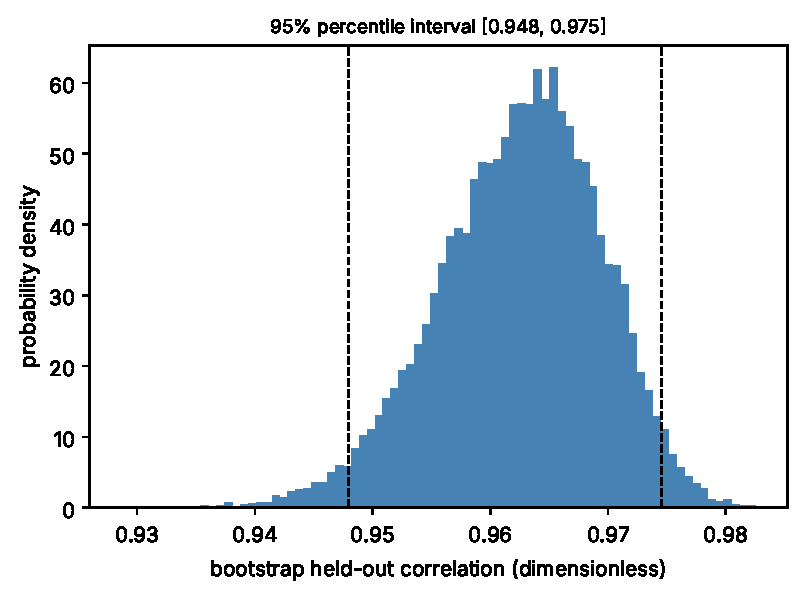
\includegraphics[width=0.85\linewidth]{figs/controls_oraclecorr.pdf}
\caption{Bootstrap distribution of the held-out correlation between the six-prime explicit-formula prediction and the true fluctuations of zeros 401--500 ($2\times10^4$ resamples of the 100 levels, seed 1). Vertical lines: the $2.5\%$ and $97.5\%$ percentiles, which agree with the paper's interval $[+0.95,+0.97]$ (Table~V caption) to within $0.01$.}\label{fig:controls-oraclecorr}
\end{figure}

\subsection{What a held-out bootstrap measures, and what it does not}

Be precise about the question the bootstrap answers in the paper. The model has already been fitted; its predictions for levels 401--500 are fixed numbers. Resampling the held-out levels asks: \emph{if the score had been computed on a different set of 100 levels behaving like these, how much would it move?} It treats the held-out levels as a sample from a conceptual population of ``levels at this height''. The zeros themselves are not random; they are fixed numbers determined by the zeta function. The randomness is a modeling device that lets us express how representative a finite window is.

The held-out bootstrap does \emph{not} include: variability from a different training set; variability from the optimizer (different random starts); or variability from a different choice of basis size. Those are probed by other means (Sec.~\ref{sec:controls-ensembles}).

\begin{pitfall}
Resample \emph{pairs}, not the two columns separately. If you resample the true fluctuations and the predictions independently, you destroy their association, and the bootstrap correlation scatters around zero whatever the model's skill. Step 4 of the last Sample Problem keeps each prediction attached to its own level.
\end{pitfall}

\begin{checkpoint}
A model's held-out rms is $0.369$ with bootstrap interval $[0.32,0.42]$, and the null's rms on the same levels is $0.263$. Does the interval say the model is worse than the null?
\end{checkpoint}
\checkanswer{It says the model's rms is unlikely to be as low as $0.263$ on comparable levels: the whole interval lies above the null value. Strictly, a paired comparison (bootstrapping the difference of the two rms values on the same resamples) is cleaner, because the null's rms also varies from resample to resample; Problem~24 explores this.}

\begin{keyideas}
\item The bootstrap replaces the unknown distribution by the empirical one and reruns the sampling experiment by resampling with replacement.
\item For the mean, the ideal bootstrap variance is exactly $\hat\sigma^2/n$ (Eq.~\eqref{eq:controls-bootvarmean}).
\item Percentile intervals take quantiles of the bootstrap replicates; they are approximate and need $n$ not too small.
\item A held-out bootstrap measures uncertainty due to which levels were scored, nothing else.
\end{keyideas}

%======================================================================
\section{When neighbors are correlated}\label{sec:controls-serial}

The bootstrap of Sec.~\ref{sec:controls-bootstrap} assumes independence. The fluctuations of consecutive zeros are \emph{not} independent: Chapter~\ref{ch:generalization} showed (and the paper's Sec.~III states) that they have negative autocorrelation at lags 1--3. How much does dependence change the standard error?

\subsection{Variance of the mean of a correlated sequence}

Model the sequence as \textbf{stationary}: every $X_j$ has the same mean $\mu$ and variance $\gamma_0$, and the covariance between two terms depends only on their separation,
\begin{equation}
\gamma_k=\mathrm{Cov}(X_j,X_{j+k}),\qquad \rho_k=\gamma_k/\gamma_0 .
\label{eq:controls-autocov}
\end{equation}
Here $\gamma_k$ is the \textbf{autocovariance} at lag $k$ and $\rho_k$ the \textbf{autocorrelation} (Chapter~\ref{ch:probability}). Repeat the first three lines of Eq.~\eqref{eq:controls-varmean}, but now keep the off-diagonal terms:
\begin{align}
\mathrm{Var}(\bar X)&=\frac1{n^2}\sum_{i=1}^n\sum_{j=1}^n\gamma_{|i-j|}.
\label{eq:controls-doublesum}
\end{align}
Count how many index pairs $(i,j)$ have $|i-j|=k$. For $k=0$ there are $n$ pairs ($i=j$). For $1\le k\le n-1$, the pairs with $j=i+k$ need $1\le i\le n-k$, giving $n-k$ pairs, and the pairs with $i=j+k$ give another $n-k$. So
\begin{align}
\mathrm{Var}(\bar X)&=\frac1{n^2}\Big[n\gamma_0+2\sum_{k=1}^{n-1}(n-k)\gamma_k\Big]\nonumber\\
&=\frac{\gamma_0}{n}\Big[1+2\sum_{k=1}^{n-1}\Big(1-\frac kn\Big)\rho_k\Big]\quad\text{(factor out $n\gamma_0$)}\nonumber\\
&\equiv\frac{\gamma_0}{n}\,f_n .
\label{eq:controls-varcorr}
\end{align}
The number $f_n$ is the \textbf{variance inflation factor}. Independent data have all $\rho_k=0$ and $f_n=1$, recovering Eq.~\eqref{eq:controls-varmean}. Positive correlations make $f_n>1$ (the data are partly redundant); negative correlations make $f_n<1$ (errors cancel between neighbors). The \textbf{effective sample size} is
\begin{equation}
n_{\rm eff}=n/f_n,
\label{eq:controls-neff}
\end{equation}
the number of independent observations that would give the same variance of the mean.

\subsection{A worked model: the AR(1) sequence}

The simplest correlated sequence is the \textbf{autoregressive process of order one}, AR(1):
\begin{equation}
X_j=\varphi X_{j-1}+e_j,\qquad |\varphi|<1,
\label{eq:controls-ar1}
\end{equation}
where the $e_j$ are independent, with mean zero and variance $\sigma_e^2$, and $e_j$ is independent of all earlier $X$. Each term remembers a fraction $\varphi$ of the previous one and adds fresh noise.

\emph{Variance.} Take the variance of both sides of Eq.~\eqref{eq:controls-ar1}. The two terms on the right are independent, so their variances add: $\gamma_0=\varphi^2\gamma_0+\sigma_e^2$ (stationarity: $\mathrm{Var}(X_{j-1})=\mathrm{Var}(X_j)=\gamma_0$). Solving,
\begin{equation}
\gamma_0=\frac{\sigma_e^2}{1-\varphi^2}.
\label{eq:controls-ar1var}
\end{equation}

\emph{Autocovariance.} Take $\mu=0$ (it does not affect covariances). Multiply Eq.~\eqref{eq:controls-ar1} by $X_{j-k}$ for $k\ge1$ and take expectations:
\begin{equation}
E[X_jX_{j-k}]=\varphi\,E[X_{j-1}X_{j-k}]+E[e_jX_{j-k}].
\end{equation}
The last term vanishes because $e_j$ is independent of the earlier $X_{j-k}$ and has mean zero. The left side is $\gamma_k$ and the first term on the right is $\varphi\gamma_{k-1}$. So $\gamma_k=\varphi\gamma_{k-1}$, and applying this $k$ times,
\begin{equation}
\gamma_k=\varphi^k\gamma_0,\qquad\rho_k=\varphi^k.
\label{eq:controls-ar1rho}
\end{equation}

\emph{Inflation factor for large $n$.} When $n$ is large, the weights $1-k/n$ are close to 1 for all $k$ where $\varphi^k$ is not negligible, so
\begin{equation}
f_\infty=1+2\sum_{k=1}^\infty\varphi^k=1+\frac{2\varphi}{1-\varphi}=\frac{1+\varphi}{1-\varphi},
\label{eq:controls-finf}
\end{equation}
using the geometric series $\sum_{k\ge1}\varphi^k=\varphi/(1-\varphi)$ (Chapter~\ref{ch:series}).

\emph{Inflation factor for finite $n$.} We need also $\sum_{k\ge1}k\varphi^k$. Call it $S$. Then $\varphi S=\sum_{k\ge1}k\varphi^{k+1}=\sum_{k\ge2}(k-1)\varphi^k$. Subtracting term by term,
\begin{equation}
S-\varphi S=\sum_{k\ge1}\big[k-(k-1)\big]\varphi^k=\sum_{k\ge1}\varphi^k=\frac{\varphi}{1-\varphi},
\qquad\text{so}\qquad S=\frac{\varphi}{(1-\varphi)^2}.
\label{eq:controls-kphik}
\end{equation}
Next, replace the finite sums $\sum_{k=1}^{n-1}$ by infinite ones. This adds the tail $\sum_{k\ge n}(1-k/n)\varphi^k$. Write $k=n+j$, so that $\abs{1-k/n}=j/n$. The magnitude of the tail is then at most $\sum_{j\ge0}(j/n)\abs{\varphi}^{n+j}=\frac{\abs{\varphi}^{n+1}}{n(1-\abs{\varphi})^2}$, using Eq.~\eqref{eq:controls-kphik} with $\abs{\varphi}$ in place of $\varphi$. This is negligible when $\abs{\varphi}^n\ll1$. Making the replacement,
\begin{equation}
f_n\approx1+2\Big[\frac{\varphi}{1-\varphi}-\frac1n\,\frac{\varphi}{(1-\varphi)^2}\Big].
\label{eq:controls-fn}
\end{equation}

\begin{sample}{How much does correlation change the error bar?}
An AR(1) sequence has $n=200$ terms. Find $f_n$, the factor by which the true SE of the mean differs from the naive $\sqrt{\gamma_0/n}$, and $n_{\rm eff}$, for (a) $\varphi=0.5$ and (b) $\varphi=-0.5$.

\textbf{Step 1 (a):} $\varphi/(1-\varphi)=0.5/0.5=1$ and $\varphi/(1-\varphi)^2=0.5/0.25=2$.

\textbf{Step 2 (a):} Eq.~\eqref{eq:controls-fn}: $f_{200}=1+2[1-2/200]=1+2(0.99)=2.98$. SE ratio $\sqrt{2.98}=1.726$. $n_{\rm eff}=200/2.98=67.1$.

\textbf{Step 3 (b):} $\varphi/(1-\varphi)=-0.5/1.5=-1/3$ and $\varphi/(1-\varphi)^2=-0.5/2.25=-0.2222$.

\textbf{Step 4 (b):} $f_{200}=1+2[-0.33333+0.2222/200]=1+2(-0.33222)=0.3356$. SE ratio $\sqrt{0.3356}=0.579$. $n_{\rm eff}=200/0.3356=596$.

\[
\boxed{\text{(a) }f=2.98,\ n_{\rm eff}=67;\qquad\text{(b) }f=0.336,\ n_{\rm eff}=596}
\]
The large-$n$ limits from Eq.~\eqref{eq:controls-finf} are $3$ and $1/3$. Positive correlation makes 200 points worth 67; negative correlation makes them worth nearly 600, \emph{for the mean}.
\end{sample}

\subsection{What the independent bootstrap gets wrong}

The independent bootstrap resamples points as if they were iid. Inside the bootstrap world the resampled points really are independent, so it reports $\sqrt{\hat\sigma^2/n}\approx\sqrt{\gamma_0/n}$ and misses the factor $\sqrt{f_n}$ entirely. With positive correlation the bootstrap interval is too narrow (overconfident); with negative correlation it is too wide (conservative). Figure~\ref{fig:controls-ar1} shows sample paths and the size of the effect.

For the paper, two cautions apply. First, the zero fluctuations are negatively correlated at short lags, which for the \emph{mean} would make the independent bootstrap conservative. Second, the paper's scores are rms errors and correlations of prediction errors, not means of the fluctuations, and Eq.~\eqref{eq:controls-varcorr} does not apply to them directly. The paper did not guess: it reran the intervals with a block bootstrap and reports that they ``widen slightly and no conclusion changes'' (Sec.~III). The next section explains the method.

\begin{figure}[htbp]\centering
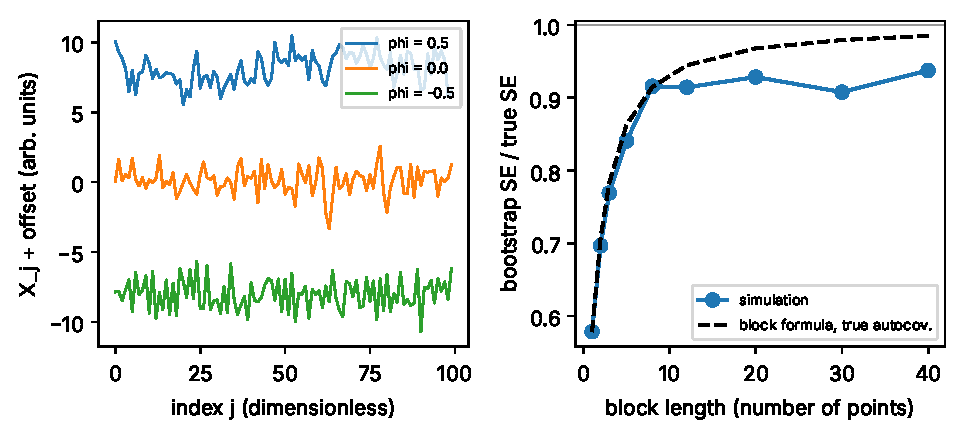
\includegraphics[width=\linewidth]{figs/controls_ar1.pdf}
\caption{Left: sample paths of AR(1) sequences (Eq.~\eqref{eq:controls-ar1}, unit noise variance) with $\varphi=0.5$, $0$ and $-0.5$, offset vertically. Positive $\varphi$ gives slow wandering; negative $\varphi$ gives zig-zag. Right: for $\varphi=0.5$, $n=400$, the average circular-block-bootstrap standard error of the mean divided by the true one (Eq.~\eqref{eq:controls-varcorr}), against block length $\ell$ (40 simulated series, 300 resamples each). $\ell=1$ is the independent bootstrap, short by about the factor $1/\sqrt{f_n}$. The dashed curve is the exact block formula Eq.~\eqref{eq:controls-cbbvar} evaluated with the true autocovariances.}\label{fig:controls-ar1}
\end{figure}

\begin{checkpoint}
Consecutive spacings between zeros are anticorrelated. Would the independent bootstrap overstate or understate the uncertainty of the \emph{mean} fluctuation of a block of zeros?
\end{checkpoint}
\checkanswer{Overstate. Negative short-lag autocorrelation gives $f_n<1$ in Eq.~\eqref{eq:controls-varcorr}, so the true variance of the mean is smaller than the independent formula.}

\begin{keyideas}
\item For a stationary sequence, $\mathrm{Var}(\bar X)=(\gamma_0/n)f_n$ with $f_n=1+2\sum_k(1-k/n)\rho_k$ (Eq.~\eqref{eq:controls-varcorr}).
\item AR(1): $\rho_k=\varphi^k$ and $f_\infty=(1+\varphi)/(1-\varphi)$.
\item The independent bootstrap ignores $f_n$: overconfident for positive, conservative for negative correlation (for the mean).
\end{keyideas}

%======================================================================
\section{The block bootstrap}\label{sec:controls-block}

\subsection{Resampling blocks instead of points}

If short-range dependence is the problem, keep short stretches of the data intact. Choose a \textbf{block length} $\ell$, cut the sequence into overlapping blocks of $\ell$ consecutive observations, and resample whole blocks.

\textbf{Moving block bootstrap.} The blocks are $\mathcal B_j=(x_j,x_{j+1},\dots,x_{j+\ell-1})$ for $j=1,\dots,n-\ell+1$. Draw $b=\lceil n/\ell\rceil$ blocks uniformly with replacement, concatenate them, and keep the first $n$ values.

\textbf{Circular block bootstrap.} Wrap the data around a circle, so that after $x_n$ comes $x_1$ again. Now a block can start at any $j=1,\dots,n$, and its entries are $x_{j},x_{j+1},\dots$ with indices taken modulo $n$. Resampling proceeds as before.

Figure~\ref{fig:controls-blocks} draws both for $n=12$, $\ell=3$. Inside each block the original neighbors stay neighbors, so the block carries the short-range correlations; only at the joins between blocks is the order broken. These methods were introduced and analyzed in the 1980s and 1990s (the moving block version by H.~K\"unsch, the circular version by D.~Politis and J.~Romano).

\begin{figure}[htbp]\centering
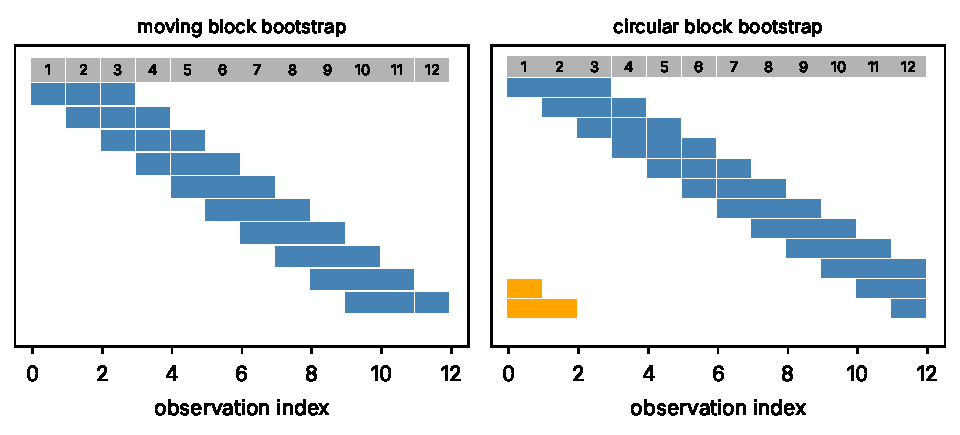
\includegraphics[width=\linewidth]{figs/controls_blocks.pdf}
\caption{Blocks of length $\ell=3$ for $n=12$ observations (gray boxes, numbered). Each row below is one block available for resampling. Left: the moving block bootstrap has $n-\ell+1=10$ blocks, so observations near the ends belong to fewer blocks. Right: the circular block bootstrap wraps around (orange cells), giving $n=12$ blocks and putting every observation in exactly $\ell$ of them.}\label{fig:controls-blocks}
\end{figure}

\begin{sample}{Counting blocks}
A held-out set has $n=100$ levels and the block length is $\ell=5$. (a) How many blocks are available in each method, and how many are drawn per resample? (b) In the moving block version, how many blocks contain observation 1, observation 3, and observation 50? (c) What is the expected number of copies of observation 1 and of observation 50 in one resample, in each method?

\textbf{Step 1 (a):} Moving: $n-\ell+1=96$ blocks. Circular: $n=100$. Drawn per resample: $\lceil100/5\rceil=20$.

\textbf{Step 2 (b):} Observation $i$ lies in block $\mathcal B_j$ when $j\le i\le j+4$, i.e.\ $i-4\le j\le i$, and also $1\le j\le96$. The count is $\min(i,96)-\max(1,i-4)+1$. For $i=1$: $1-1+1=1$. For $i=3$: $3-1+1=3$. For $i=50$: $50-46+1=5$.

\textbf{Step 3 (c), moving:} Each drawn block contains observation $i$ with probability (number of blocks containing $i$)/96, and contributes one copy when it does. Twenty independent blocks give expected copies $20\times1/96=0.208$ for $i=1$ and $20\times5/96=1.042$ for $i=50$.

\textbf{Step 4 (c), circular:} Every observation is in exactly 5 of the 100 blocks: expected copies $20\times5/100=1$ for every $i$.

\[
\boxed{\text{moving: }0.208\text{ vs }1.042\text{ copies};\quad\text{circular: }1\text{ copy for every observation}}
\]
The moving version under-represents the ends; the circular version treats every observation equally, which is why it is often preferred.
\end{sample}

\subsection{What the block bootstrap does to the variance of a mean}

For the mean we can compute the circular block bootstrap variance exactly, which shows what the method captures. Assume $n=b\ell$ exactly, so $b$ blocks fill the resample with no truncation.

\textbf{Step (i).} The bootstrap mean is the average of the $b$ block means: $\bar x^*=\frac1b\sum_{i=1}^b\bar{\mathcal B}^*_i$, where $\bar{\mathcal B}^*_i$ is the mean of the $i$-th drawn block.

\textbf{Step (ii).} The drawn blocks are independent, so $\mathrm{Var}^*(\bar x^*)=\frac1b\mathrm{Var}^*(\bar{\mathcal B}^*)$ (Eq.~\eqref{eq:controls-varmean} with $b$ terms).

\textbf{Step (iii).} A drawn block mean equals $\bar{\mathcal B}_j$ with probability $1/n$ for each start $j$. The average of the $\bar{\mathcal B}_j$ over $j$ is $\bar x$, because every observation sits in exactly $\ell$ blocks with weight $1/\ell$ in each. Hence $\mathrm{Var}^*(\bar{\mathcal B}^*)=\frac1n\sum_{j=1}^n(\bar{\mathcal B}_j-\bar x)^2$.

\textbf{Step (iv).} Write $y_j=x_j-\bar x$ (indices modulo $n$). Then $\bar{\mathcal B}_j-\bar x=\frac1\ell\sum_{a=0}^{\ell-1}y_{j+a}$ and
\begin{equation}
\frac1n\sum_{j=1}^n(\bar{\mathcal B}_j-\bar x)^2=\frac1{\ell^2}\sum_{a=0}^{\ell-1}\sum_{c=0}^{\ell-1}\Big[\frac1n\sum_{j=1}^ny_{j+a}y_{j+c}\Big]=\frac1{\ell^2}\sum_{a,c}\tilde\gamma_{|c-a|},
\end{equation}
where $\tilde\gamma_k=\frac1n\sum_{j=1}^ny_jy_{j+k}$ is the \textbf{circular sample autocovariance}. (Shifting the summation index $j$ around the circle does not change the inner sum, so it depends only on $c-a$; and $\tilde\gamma_k=\tilde\gamma_{-k}$.)

\textbf{Step (v).} Counting pairs $(a,c)$ with $|c-a|=k$ exactly as in Eq.~\eqref{eq:controls-varcorr}, but with $\ell$ in place of $n$:
$\frac1{\ell^2}\sum_{a,c}\tilde\gamma_{|c-a|}=\frac1\ell\big[\tilde\gamma_0+2\sum_{k=1}^{\ell-1}(1-k/\ell)\tilde\gamma_k\big]$.

\textbf{Step (vi).} Combine with (ii) and $b=n/\ell$:
\begin{equation}
\mathrm{Var}^*_{\rm CBB}(\bar x^*)=\frac1n\Big[\tilde\gamma_0+2\sum_{k=1}^{\ell-1}\Big(1-\frac k\ell\Big)\tilde\gamma_k\Big].
\label{eq:controls-cbbvar}
\end{equation}

Compare with Eq.~\eqref{eq:controls-varcorr}. The block bootstrap uses the data's own autocovariances up to lag $\ell-1$, with weights $1-k/\ell$ instead of $1-k/n$, and drops all lags $\ge\ell$. For $\ell=1$ it reduces to $\tilde\gamma_0/n=\hat\sigma^2/n$, the independent bootstrap. Two consequences follow:
\begin{itemize}
\item $\ell$ must be longer than the range over which correlations matter, or they are cut off (bias).
\item $\ell$ must be much shorter than $n$, so that there are many blocks to resample (otherwise the estimate is noisy, and the weights $1-k/\ell$ still discount real correlations).
\end{itemize}
For the AR(1) with $\varphi=0.5$, $n=400$ and $\ell=20$, inserting the true autocovariances into Eq.~\eqref{eq:controls-cbbvar} gives a factor $1+2(1-2/20)=2.8$ instead of the true $f_{400}=1+2(1-2/400)=2.99$ (Eq.~\eqref{eq:controls-fn}), so the block standard error is about $3\%$ low, while the independent bootstrap is about $42\%$ low (factor $1/\sqrt{2.99}=0.578$). The right panel of Fig.~\ref{fig:controls-ar1} compares these predictions with a simulation. The simulated ratios sit close to the dashed curve, slightly below it, because the bootstrap uses autocovariances measured about the sample mean.

In practice nobody knows the right $\ell$, so the honest procedure is to report a range: compute intervals for several block lengths and check whether conclusions change. That is exactly what the paper does with ``block lengths 3 to 20'' (Sec.~III; Appendix~A step 22).

\begin{pycode}
import numpy as np

def cbb_indices(n, ell, rng):
    """Positions for one circular-block-bootstrap resample."""
    nb = -(-n // ell)                       # ceil(n / ell) blocks
    starts = rng.integers(0, n, nb)         # any start; wrap around
    idx = (starts[:, None] + np.arange(ell)[None, :]) % n
    return idx.ravel()[:n]                  # truncate to length n

rng = np.random.default_rng(2)
x = rng.normal(size=100)                    # stand-in data
reps = [x[cbb_indices(100, 5, rng)].mean() for _ in range(5000)]
print(np.std(reps))
\end{pycode}

\begin{beyond}
For stationary sequences whose correlations die out fast enough, the moving and circular block bootstraps are consistent provided $\ell\to\infty$ and $\ell/n\to0$ as $n\to\infty$. The proofs, and rules for choosing $\ell$ (it should grow roughly like $n^{1/3}$ for variance estimation), are in the specialized literature and beyond this book. For $n=100$ held-out levels and correlations lasting a few lags, block lengths 3 to 20 bracket every sensible choice.
\end{beyond}

\begin{pitfall}
A block bootstrap on $n=100$ points with $\ell=20$ draws only five blocks per resample. Its replicates are then made from a handful of pieces and the interval can be erratic. Report a range of $\ell$, not one hand-picked value.
\end{pitfall}

\begin{checkpoint}
What does the circular block bootstrap with $\ell=1$ reduce to?
\end{checkpoint}
\checkanswer{The ordinary independent bootstrap: blocks of one point resampled with replacement. Eq.~\eqref{eq:controls-cbbvar} then gives $\tilde\gamma_0/n=\hat\sigma^2/n$, as in Eq.~\eqref{eq:controls-bootvarmean}.}

\begin{keyideas}
\item Block bootstraps resample stretches of $\ell$ consecutive points, preserving dependence within blocks.
\item The circular version wraps around so every point appears in exactly $\ell$ blocks.
\item For the mean, the circular block variance is Eq.~\eqref{eq:controls-cbbvar}: autocovariances up to lag $\ell-1$, Bartlett-weighted.
\item Choose $\ell$ longer than the correlation range, much shorter than $n$; report sensitivity over a range.
\end{keyideas}

%======================================================================
\section{Permutation tests}\label{sec:controls-permutation}

Uncertainty intervals tell you how precisely a score is known. A different kind of question is: \emph{could this result have arisen if there were no effect at all?} Statistics answers it with a test.

\subsection{The vocabulary of a test}

\begin{itemize}
\item The \textbf{null hypothesis} $H_0$ is a precise statement of ``no effect'', precise enough that you can compute (or simulate) what data would look like under it.
\item The \textbf{test statistic} $T$ is a number computed from the data that tends to be large when there is an effect.
\item The \textbf{p-value} is the probability, computed assuming $H_0$, of a statistic at least as extreme as the one observed: $p=P_{H_0}(T\ge T_{\rm obs})$.
\end{itemize}
A small $p$ means the data would be surprising under $H_0$. It is \emph{not} the probability that $H_0$ is true; it is a statement about data given a hypothesis.

\subsection{Exchangeability and the permutation idea}

A \textbf{permutation test} (introduced by R.~A.~Fisher in the 1930s) builds the null distribution from the data themselves. Suppose $H_0$ says that some labels attached to the data are irrelevant: for example, ``treatment'' and ``control'' labels in an experiment, or the pairing between a prediction and a true value. Then under $H_0$ every rearrangement of the labels was equally likely to have produced the data we see. This property is called \textbf{exchangeability}. Computing $T$ for every rearrangement gives the exact distribution of $T$ under $H_0$, and the p-value is the fraction of rearrangements with $T\ge T_{\rm obs}$.

\begin{sample}{An exact permutation test}
Group A has values $(3,6,8)$ and group B has $(1,2,4)$. Test $H_0$: ``the group labels are irrelevant'' with statistic $D=\bar x_A-\bar x_B$.

\textbf{Step 1:} Observed: $\bar x_A=17/3$, $\bar x_B=7/3$, $D_{\rm obs}=10/3=3.333$.

\textbf{Step 2:} Pool the six values $\{1,2,3,4,6,8\}$, total $24$. Under $H_0$ any 3 of the 6 could have been group A: $\binom63=20$ equally likely relabelings.

\textbf{Step 3:} If group A has sum $S_A$, then $D=\frac{S_A-(24-S_A)}{3}=\frac{2S_A-24}{3}$. So $D\ge10/3$ exactly when $S_A\ge17$.

\textbf{Step 4:} Three-element subsets with sum $\ge17$: $\{4,6,8\}$ (18) and $\{3,6,8\}$ (17). The next largest, $\{2,6,8\}$, has 16. Two subsets.

\textbf{Step 5:} One-sided $p=2/20=0.1$. For a two-sided test count also $D\le-10/3$, i.e.\ $S_A\le7$: $\{1,2,3\}$ (6) and $\{1,2,4\}$ (7). Two-sided $p=4/20=0.2$.

\[
\boxed{p_{\text{one-sided}}=0.10,\qquad p_{\text{two-sided}}=0.20}
\]
With three values per group, even a clear-looking separation is not surprising: one relabeling in ten does as well.
\end{sample}

\subsection{Testing a correlation}

To test whether a prediction $a_j$ is associated with the truth $b_j$, take $H_0$: ``the pairing is irrelevant''. Randomly permute the $b_j$ among the levels, recompute the correlation, and repeat. The fraction of permuted correlations at least as large as the observed one is the p-value.

Be careful about what this $H_0$ includes. Permuting the $b_j$ assumes that, absent association, \emph{every} ordering of the $b_j$ was equally likely. If the true fluctuations are serially correlated (they are) and the predictions are smooth (fitted potentials produce smooth level shifts), then unpermuted pairs share slow trends that random permutations destroy. A permutation test can then report ``significant'' association produced by shared serial structure rather than by skill. The cure is the same as for the bootstrap: respect the dependence (for example, by circularly shifting one sequence relative to the other instead of shuffling it), or use surrogates that preserve the serial structure (Sec.~\ref{sec:controls-surrogates}).

\subsection{Monte Carlo tests and the size of an ensemble}

Usually there are too many rearrangements to enumerate, so we draw $N$ random ones (or $N$ surrogate data sets). Let $r$ be the number of them whose statistic is at least $T_{\rm obs}$. The Monte Carlo p-value is
\begin{equation}
p=\frac{1+r}{N+1}.
\label{eq:controls-mcp}
\end{equation}
\emph{Why $1+r$ over $N+1$?} Under $H_0$, the real data and the $N$ simulated ones are generated by the same mechanism, so the real statistic is equally likely to have any of the $N+1$ ranks in the combined list (ignoring ties). The probability that it ranks among the top $r+1$ is therefore $(r+1)/(N+1)$. This is the probability of a result at least as extreme as the one observed, which is the definition of $p$.

An immediate consequence: \textbf{the smallest p-value an ensemble of size $N$ can ever produce is $1/(N+1)$}. Even if no simulated statistic comes close, you can claim no more.

\begin{sample}{What an ensemble of 200 can show}
A statistic is computed on real data and on 200 surrogate data sets; none of the 200 reaches the real value. What is the Monte Carlo p-value? If the surrogates had numbered 100?

\textbf{Step 1:} $r=0$, $N=200$: $p=1/201=0.004975$.

\textbf{Step 2:} $N=100$: $p=1/101=0.0099$.

\textbf{Step 3:} Interpretation: the result is limited by the ensemble size, not by how far the real value is from the surrogates. To claim $p<10^{-4}$ you need at least $10^4$ surrogates.

\[
\boxed{p\le1/201\approx0.005\ \ (N=200),\qquad p\le1/101\approx0.010\ \ (N=100)}
\]
\end{sample}

\begin{pitfall}
``$p=0.01$'' does not mean ``the null hypothesis has a $1\%$ chance of being true'', nor ``the effect is large''. It means that data this extreme would arise in about $1\%$ of experiments \emph{if} $H_0$ held. And it is only meaningful if the test was chosen before seeing the data (Sec.~\ref{sec:controls-posthoc}).
\end{pitfall}

\begin{checkpoint}
In a permutation test of a correlation, which hypothesis is being tested: ``the model has no skill'' or ``the truth values are exchangeable with respect to the predictions''?
\end{checkpoint}
\checkanswer{The second. ``No skill'' is translated into exchangeability. If exchangeability fails for another reason (serial correlation), the test can reject even when the model has no skill.}

\begin{keyideas}
\item A test needs a precise null hypothesis, a statistic, and a p-value $P_{H_0}(T\ge T_{\rm obs})$.
\item Permutation tests generate the null distribution by rearranging labels; they test exchangeability.
\item Monte Carlo p-value: $(1+r)/(N+1)$; an ensemble of size $N$ cannot show $p<1/(N+1)$.
\end{keyideas}

%======================================================================
\section{Surrogate data}\label{sec:controls-surrogates}

\subsection{The idea}

A permutation test destroys \emph{all} order in the data. Sometimes that is too much: you want to destroy one specific property while keeping others. \textbf{Surrogate data} are synthetic data sets constructed to share chosen properties $\mathcal P$ with the real data while lacking a property $\mathcal Q$ under investigation \cite{theiler}. The null hypothesis becomes: ``the real data are a typical member of the class of sequences with properties $\mathcal P$''. If an analysis cannot tell the real data from their surrogates, then whatever it measures is explained by $\mathcal P$ alone and is not evidence for $\mathcal Q$.

We describe three families, each preserving different things. Throughout, $d_1,\dots,d_n$ is a real sequence, for instance the fluctuations of zeros in mean spacings.

\subsection{Random permutation}

Reorder $d_1,\dots,d_n$ randomly. The \textbf{marginal distribution} (the histogram of values, ignoring order) is preserved exactly, because the surrogate contains the very same numbers. All serial structure is destroyed: on average the surrogate's autocorrelation at any nonzero lag is close to zero (precisely, $-1/(n-1)$ for a mean-zero sequence; Problem~8).

\subsection{Phase randomization}

Recall from Chapter~\ref{ch:fourier-transform} the DFT of a length-$n$ sequence,
\begin{equation}
D_q=\sum_{j=0}^{n-1}d_j\,e^{-2\pi i jq/n},\qquad d_j=\frac1n\sum_{q=0}^{n-1}D_q\,e^{2\pi i jq/n},
\label{eq:controls-dft}
\end{equation}
(indices from $0$ here, as in \texttt{numpy}). For real $d$, replacing $q$ by $n-q$ gives $e^{-2\pi i j(n-q)/n}=e^{-2\pi ij}e^{2\pi ijq/n}=e^{2\pi ijq/n}$, so
\begin{equation}
D_{n-q}=D_q^*,
\label{eq:controls-hermsym}
\end{equation}
where the star is the complex conjugate. In particular $D_0=\sum_jd_j$ is real, and for even $n$, $D_{n/2}=\sum_j(-1)^jd_j$ is real.

The \textbf{phase-randomized surrogate} (Theiler and co-workers \cite{theiler}) multiplies each $D_q$ by a random phase factor $e^{i\phi_q}$, $\phi_q$ uniform in $[0,2\pi)$, with two constraints that keep the result real: $\phi_{n-q}=-\phi_q$ (so Eq.~\eqref{eq:controls-hermsym} still holds), and $\phi_0=0$ (and $\phi_{n/2}=0$ for even $n$), so the real coefficients stay real. Then invert the DFT. Every magnitude $|D_q|$ is unchanged.

\emph{What is preserved.} The mean (because $D_0$ is untouched), the power spectrum $|D_q|^2$ by construction, and hence the circular autocorrelation. To see the last claim, define the circular autocorrelation $c_k=\sum_{j=0}^{n-1}d_jd_{(j+k)\bmod n}$ and compute its DFT:
\begin{align}
C_q&=\sum_{k=0}^{n-1}c_k\,e^{-2\pi ikq/n}=\sum_{j=0}^{n-1}d_j\sum_{k=0}^{n-1}d_{(j+k)\bmod n}\,e^{-2\pi ikq/n}.
\end{align}
Put $l=(j+k)\bmod n$. As $k$ runs over $0,\dots,n-1$ with $j$ fixed, $l$ runs over the same values once each, and $e^{-2\pi ikq/n}=e^{-2\pi i(l-j)q/n}$ (adding a multiple of $n$ to the exponent's numerator changes nothing, since $e^{-2\pi i q}=1$). So
\begin{equation}
C_q=\Big(\sum_{j}d_je^{2\pi ijq/n}\Big)\Big(\sum_{l}d_le^{-2\pi ilq/n}\Big)=D_q^*D_q=|D_q|^2 .
\label{eq:controls-wk}
\end{equation}
This is the discrete Wiener--Khinchin theorem of Chapter~\ref{ch:fourier-transform}. Since $c_k$ is recovered from $C_q$ by the inverse DFT, two sequences with the same $|D_q|$ have the same circular autocorrelation at every lag. By Parseval's theorem, $\sum_jd_j^2=c_0=\frac1n\sum_q|D_q|^2$, so the variance is preserved too.

\emph{What is destroyed.} The specific phases: \emph{where} each oscillation is at each index, and how oscillations at different frequencies line up. A sawtooth, for example, owes its shape to harmonics locked in phase; randomizing the phases turns it into a smooth, irregular wiggle with the same spectrum. The marginal distribution generally changes; a sum of many components with random phases tends to look Gaussian (a consequence of the central limit theorem, which we do not prove).

\begin{sample}{Phase randomization by hand}
Let $d=(1,2,0,-1)$, $n=4$. Compute its DFT, rotate the phase of $D_1$ by $\phi=\pi/4$ (and $D_3$ by $-\pi/4$), invert, and check that the circular autocorrelation is unchanged.

\textbf{Step 1:} With $n=4$, $e^{-2\pi ijq/4}=(-i)^{jq}$. $D_0=1+2+0-1=2$. $D_2=1-2+0+1=0$. $D_1=1+2(-i)+0(-1)+(-1)(i)=1-3i$. $D_3=D_1^*=1+3i$.

\textbf{Step 2:} For real $d$ with these symmetries the inverse DFT simplifies to $d_j=\frac14[D_0+2\,\Re(D_1i^j)+D_2(-1)^j]$. Check: $j=1$: $D_1i=i+3$, real part $3$, $d_1=\frac14(2+6)=2$. Correct.

\textbf{Step 3:} New coefficient $D_1'=(1-3i)e^{i\pi/4}=(1-3i)\frac{1+i}{\sqrt2}=\frac{1+i-3i+3}{\sqrt2}=\frac{4-2i}{\sqrt2}=2\sqrt2-\sqrt2\,i$. Its magnitude is $\sqrt{8+2}=\sqrt{10}=|D_1|$.

\textbf{Step 4:} Write $D_1'=a+ib$ with $a=2\sqrt2$, $b=-\sqrt2$. Then $\Re(D_1'i^j)$ is $a,\,-b,\,-a,\,b$ for $j=0,1,2,3$, and $d'_j=\frac14(2+2\Re(D_1'i^j))$:
\[
d'=\big(\tfrac12+\sqrt2,\ \tfrac12+\tfrac{\sqrt2}2,\ \tfrac12-\sqrt2,\ \tfrac12-\tfrac{\sqrt2}2\big)=(1.914,\ 1.207,\ -0.914,\ -0.207).
\]

\textbf{Step 5:} Autocorrelation of $d$: $c_0=1+4+0+1=6$; $c_1=d_0d_1+d_1d_2+d_2d_3+d_3d_0=2+0+0-1=1$; $c_2=d_0d_2+d_1d_3+d_2d_0+d_3d_1=0-2+0-2=-4$; $c_3=c_1=1$.

\textbf{Step 6:} Autocorrelation of $d'$: $c'_0=(\tfrac12+\sqrt2)^2+(\tfrac12+\tfrac{\sqrt2}2)^2+(\tfrac12-\sqrt2)^2+(\tfrac12-\tfrac{\sqrt2}2)^2=3.664+1.457+0.836+0.043=6.000$. The check script confirms $c'_1=1$ and $c'_2=-4$ as well.

\[
\boxed{d'=(1.914,\,1.207,\,-0.914,\,-0.207),\quad (c_0,c_1,c_2)=(6,1,-4)\text{ for both}}
\]
The values changed (the marginal is different: $\{1,2,0,-1\}$ became four irrational numbers), the mean ($\tfrac12$) and autocorrelation did not.
\end{sample}

\subsection{Amplitude-adjusted surrogates: IAAFT}

Sometimes we want a surrogate that keeps \emph{both} the marginal and the spectrum. In general no sequence other than a rearrangement of the original has exactly the original values, and almost no rearrangement has exactly the original spectrum, so both cannot usually hold at once. Schreiber and Schmitz \cite{schreiber} proposed an iteration that keeps the marginal exactly and the spectrum approximately: the \textbf{iterative amplitude-adjusted Fourier transform} (IAAFT).
\begin{enumerate}
\item Store the original Fourier magnitudes $|D_q|$ and the sorted original values.
\item Start from a random permutation $y$ of $d$.
\item \emph{Spectrum step:} take the DFT of $y$, keep its phases, replace its magnitudes by $|D_q|$, invert.
\item \emph{Rank step:} replace the smallest value of the result by the smallest original value, the second smallest by the second smallest, and so on (``rank-order remapping''). Now the values are exactly the original ones.
\item Repeat steps 3 and 4 until the spectrum stops improving (the paper uses 200 iterations, Appendix~A step 18).
\end{enumerate}
Ending on a rank step makes the marginal exact; the spectrum is then close but not exact (the paper reports agreement ``to 1\%'', Sec.~III).

\begin{pycode}
import numpy as np

def phase_randomize(d, rng):
    D = np.fft.rfft(d)                      # q = 0 .. n//2
    ph = rng.uniform(0, 2*np.pi, len(D))
    ph[0] = 0.0                             # keep the mean
    if len(d) % 2 == 0:
        ph[-1] = 0.0                        # keep Nyquist term real
    return np.fft.irfft(D * np.exp(1j*ph), n=len(d))

def iaaft(d, rng, iters=200):
    amp = np.abs(np.fft.rfft(d))
    srt = np.sort(d)
    y = rng.permutation(d)
    for _ in range(iters):
        Y = np.fft.rfft(y)
        y = np.fft.irfft(amp * np.exp(1j*np.angle(Y)), n=len(d))
        y = srt[np.argsort(np.argsort(y))]  # rank-order remap
    return y
\end{pycode}

(\texttt{np.fft.rfft} returns only $q=0,\dots,\lfloor n/2\rfloor$; \texttt{irfft} fills in the rest using Eq.~\eqref{eq:controls-hermsym}, so the constraint $\phi_{n-q}=-\phi_q$ is automatic.)

Table~\ref{tab:controls-surr} summarizes, and Fig.~\ref{fig:controls-surrogates} shows all three applied to running example RE2, the prime-2 wave. For a zero sequence, the prime-2 term alone moves the $n$-th zero to first order by $\delta$ with $\Nsm'(s_n)\delta+N^{p=2}_{\rm fl}(s_n)=0$; since $\Nsm'(s_n)=1/\gap_n$, the fluctuation in mean spacings is $\delta/\gap_n=-N^{p=2}_{\rm fl}(s_n)$, where $N^{p=2}_{\rm fl}(t)=-\frac1\pi\sum_{m=1}^3\frac{\sin(mt\log2)}{m2^{m/2}}$.

\begin{table}[htbp]\centering
\caption{What each surrogate keeps (\checkmark), keeps approximately ($\approx$), or destroys ($\times$).}\label{tab:controls-surr}
\begin{tabular}{lccc}
\toprule
property & permutation & phase-randomized & IAAFT\\
\midrule
marginal distribution (set of values) & \checkmark & $\times$ & \checkmark\\
mean and variance & \checkmark & \checkmark & \checkmark\\
power spectrum / circular autocorrelation & $\times$ & \checkmark & $\approx$\\
specific phases (where each oscillation is) & $\times$ & $\times$ & $\times$\\
\bottomrule
\end{tabular}
\end{table}

\begin{figure}[htbp]\centering
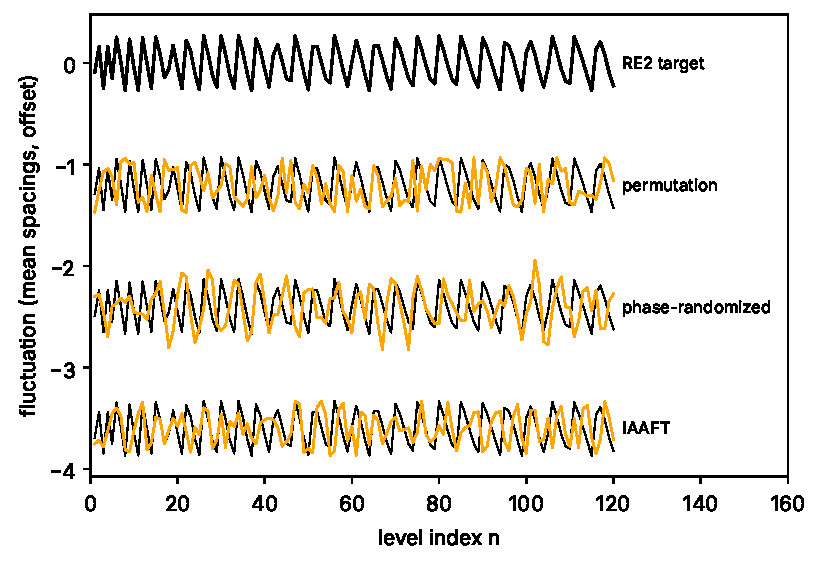
\includegraphics[width=0.9\linewidth]{figs/controls_surrogates.pdf}
\caption{Surrogates of the prime-2 target (running example RE2): the fluctuation $-N^{p=2}_{\rm fl}(s_n)$ in mean spacings for levels $n=1$--$400$ (first 120 shown, black). Orange, top to bottom: a random permutation (same values, no order), a phase-randomized surrogate (same power spectrum, new waveform), and an IAAFT surrogate (same values and nearly the same spectrum). None of the surrogates continues the black curve: the information about \emph{where} the oscillation is has been removed.}\label{fig:controls-surrogates}
\end{figure}

\begin{pitfall}
The DFT treats a sequence as one period of a periodic signal. If $d_0$ and $d_{n-1}$ are far apart, the periodic extension has a jump, the jump contributes spurious high-frequency power, and the phase-randomized surrogates inherit that power. For zero \emph{positions} (as opposed to fluctuations) there is a further constraint: a zero sequence must be increasing, which is why the paper's step 23 uses ``sorted phase-randomized surrogates''.
\end{pitfall}

\begin{checkpoint}
You want to test whether an analysis responds to the \emph{phases} of the zero fluctuations, not merely to their spectrum. Which surrogate do you use?
\end{checkpoint}
\checkanswer{A phase-randomized (or IAAFT) surrogate: it keeps the spectrum and scrambles the phases, so any difference between real and surrogate results must come from the phases.}

\begin{keyideas}
\item Surrogates keep chosen properties $\mathcal P$ and destroy a property $\mathcal Q$; the null is ``real data are typical of class $\mathcal P$''.
\item Permutation keeps the marginal; phase randomization keeps the spectrum and autocorrelation (Eq.~\eqref{eq:controls-wk}); IAAFT keeps the marginal exactly and the spectrum approximately.
\end{keyideas}

%======================================================================
\section{Controls: structure or capacity?}\label{sec:controls-capacity}

\subsection{Positive and negative controls}

In a biology laboratory, a new test for a virus is run alongside two extra samples: one known to contain the virus (a \textbf{positive control}) and one known not to (a \textbf{negative control}). If the negative control lights up, the test responds to something other than the virus; if the positive control does not light up, the test is broken. Either way you learn how to read the real result.

Computational studies need the same thing. For a fitted model:
\begin{itemize}
\item A \textbf{negative control} is a data set known to lack the structure the model is claimed to learn (a surrogate). If the model fits it as well as the real data, the fit quality is not evidence of that structure.
\item A \textbf{positive control} is a data set where the right answer is known exactly (a synthetic target with known continuation). If the model fails there, it would also fail on the real problem.
\item A \textbf{leakage control} checks that held-out data cannot influence the fit, for example by overwriting the held-out data with noise and confirming that the fitted parameters do not change.
\end{itemize}

\subsection{The logic of a surrogate refit}

Suppose a family of models reaches in-sample error $e_{\rm real}$ on the real targets. Refit the same family, with the same protocol, to surrogate targets and record $e_{\rm surr}$. Then:
\begin{itemize}
\item If $e_{\rm surr}\approx e_{\rm real}$, the family fits sequences with properties $\mathcal P$ equally well whether or not they have $\mathcal Q$. The in-sample error measures \textbf{capacity} (Chapter~\ref{ch:generalization}), not captured structure.
\item If $e_{\rm surr}\gg e_{\rm real}$, the family responds to $\mathcal Q$. This is necessary for having learned $\mathcal Q$, but not sufficient for predicting held-out data; that still requires an out-of-sample test.
\end{itemize}

\subsection{A toy demonstration}

Take the RE2 target for levels $n=101$--$200$, a sequence of 100 numbers. Fit it with two linear models by least squares (Chapter~\ref{ch:least-squares}):
\begin{itemize}
\item \textbf{Generic model:} the first $M$ functions $\cos(\pi k(j+\tfrac12)/100)$, $k=0,\dots,M-1$, of the position $j=0,\dots,99$ in the sequence. It knows nothing about primes; it is a flexible basis, like the cosine basis for $\delta V$.
\item \textbf{Structured model:} the six functions $\sin(m s_n\log2)$, $\cos(m s_n\log2)$, $m=1,2,3$, of the smooth height $s_n$. It knows the prime-2 frequencies.
\end{itemize}
Fit each to the real target, to 20 phase-randomized surrogates and to 20 permutations. Figure~\ref{fig:controls-capacity} shows the result.

\begin{figure}[htbp]\centering
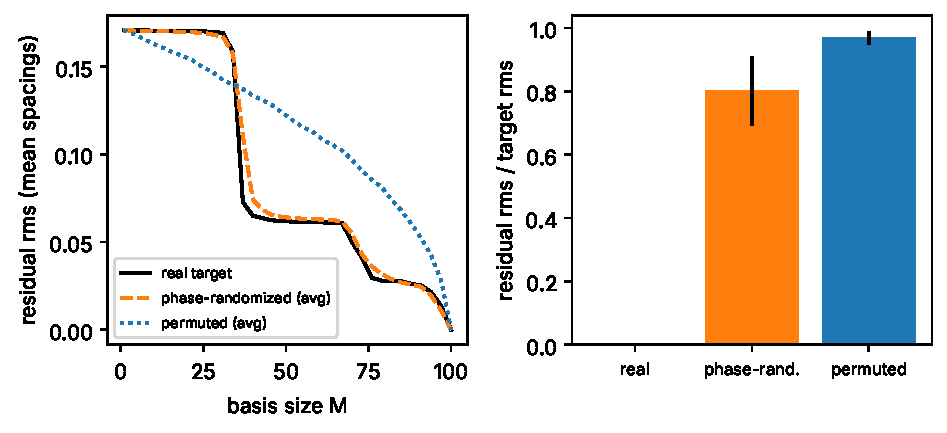
\includegraphics[width=\linewidth]{figs/controls_capacity.pdf}
\caption{In-sample fits of the prime-2 target (levels 101--200, fluctuation in mean spacings) and its surrogates. Left: residual rms of the generic cosine model against its size $M$; curves for surrogates are averages over 20 draws. All reach zero at $M=100$ (saturated), and the phase-randomized surrogates track the real target closely, because a generic basis responds mainly to the power spectrum. Right: residual rms of the six-parameter structured model, divided by the target's rms. It fits the real target exactly (the target lies in its span) and leaves most of each surrogate unexplained.}\label{fig:controls-capacity}
\end{figure}

The generic model cannot tell the real target from its phase-randomized surrogates, and at $M=100$ it fits everything exactly. Why does it treat the phase-randomized surrogates almost the same? A cosine basis in the sequence index is close to a Fourier basis, and the fraction of a target that the first $M$ basis functions capture depends on how the target's power is spread over frequency, which phase randomization preserves (this is a heuristic; the cosine and DFT bases are not identical, so the agreement is approximate). The structured model, by contrast, fits the real target to round-off precision and fails on every surrogate. Only a model with the right inductive bias makes fit quality informative.

\begin{sample}{Reading the paper's surrogate refits}
The paper (Sec.~III, ``Permutation and surrogate tests'') refits the scale-1, $M=400$ operator on zeros 1--400 to ten draws each of three surrogate families. Reported in-sample rms: permutation $0.134\pm0.010$, phase-randomized $0.141\pm0.006$, IAAFT $0.138\pm0.005$, against $0.137$ for the true zeros and $0.244$ for the null. (a) How many ``$\pm$'' units from the true-zero value is each surrogate mean? (b) What fraction of the null's error does the fit remove on the true zeros, and on each surrogate family?

\textbf{Step 1 (a):} Permutation: $(0.137-0.134)/0.010=0.3$. Phase-randomized: $(0.137-0.141)/0.006=-0.67$. IAAFT: $(0.137-0.138)/0.005=-0.2$.

\textbf{Step 2 (b):} True zeros: $1-0.137/0.244=0.439$. Permutation: $1-0.134/0.244=0.451$. Phase-randomized: $1-0.141/0.244=0.422$. IAAFT: $1-0.138/0.244=0.434$.

\[
\boxed{\text{all within }0.7\text{ spreads; the fit removes }42\text{--}45\%\text{ of the null error on every target}}
\]
The fit is equally good on sequences with no arithmetic content. The paper concludes: ``in-sample accuracy measures capacity, not captured structure.''
\end{sample}

\begin{checkpoint}
Suppose a fitted potential had reached in-sample rms $0.05$ on the true zeros but only $0.20$ on phase-randomized surrogates. Would that prove it predicts held-out zeros?
\end{checkpoint}
\checkanswer{No. It would show the family responds to the phases of the real fluctuations (necessary for having learned them), but prediction can only be established by scoring held-out zeros against the null.}

\begin{keyideas}
\item Negative controls (surrogates) test whether a result needs the structure claimed; positive controls (known answers) test whether the method can work at all; leakage controls test that held-out data cannot influence the fit.
\item If a family fits surrogates as well as real data, its in-sample quality measures capacity.
\item A generic basis responds mainly to the power spectrum; only the right inductive bias makes fit quality discriminating.
\end{keyideas}

%======================================================================
\section{Exploratory and confirmatory analysis}\label{sec:controls-posthoc}

\subsection{Two kinds of analysis}

A \textbf{confirmatory} analysis fixes the hypothesis, the statistic, the data and the decision rule \emph{before} looking at the outcome; its p-values mean what Sec.~\ref{sec:controls-permutation} says they mean. An \textbf{exploratory} analysis looks at the data, notices patterns, and invents ways to quantify them. Exploration is essential (it is how most discoveries start), but its numbers cannot be read as significance levels, because the choices that produced them were steered by the data.

\subsection{Many looks}

The simplest way the steering inflates evidence: each look at the data is a chance to be fooled. If you perform $k$ independent tests, each with false-positive probability $\alpha$ when its null is true, the probability that at least one fires is
\begin{equation}
P(\text{at least one false positive})=1-(1-\alpha)^k,
\label{eq:controls-fwer}
\end{equation}
because each test stays silent with probability $1-\alpha$ and independence multiplies these. The \textbf{Bonferroni correction} runs each test at $\alpha/k$. By the same formula, the family-wise probability is then $1-(1-\alpha/k)^k$, and this is at most $\alpha$.

To see why, use \textbf{Bernoulli's inequality}: $(1+u)^k\ge1+ku$ for $u\ge-1$ and every integer $k\ge1$. We prove it by induction.
\begin{itemize}
\item For $k=1$ it holds with equality.
\item Suppose it holds for some $k$. Then $(1+u)^{k+1}=(1+u)^k(1+u)\ge(1+ku)(1+u)=1+(k+1)u+ku^2\ge1+(k+1)u$. The first inequality multiplies both sides by $1+u\ge0$; the second drops the term $ku^2\ge0$. So it holds for $k+1$.
\end{itemize}
With $u=-\alpha/k$, Bernoulli's inequality gives $(1-\alpha/k)^k\ge1-\alpha$. Hence $1-(1-\alpha/k)^k\le\alpha$.

\begin{sample}{Twenty cutoffs}
A researcher computes a statistic for 20 different cutoffs and reports the one that crosses $p<0.05$. If none of the effects is real and the tests are independent, how often will something cross? What per-test threshold restores a $5\%$ family-wise rate?

\textbf{Step 1:} One test: $0.05$. Five tests: $1-0.95^5=1-0.7738=0.2262$.

\textbf{Step 2:} Twenty tests: $0.95^{20}=0.3585$, so $1-0.3585=0.6415$.

\textbf{Step 3:} Bonferroni: $0.05/20=0.0025$ per test, giving $1-(0.9975)^{20}=0.0488\le0.05$.

\[
\boxed{P=0.64\text{ for 20 looks};\quad\text{Bonferroni threshold }0.0025}
\]
Choosing the best of 20 cutoffs after seeing the data turns a $5\%$ false-alarm rate into roughly $64\%$. (Real cutoffs are usually correlated, which lowers this number, but in an unknown way.)
\end{sample}

\begin{figure}[htbp]\centering
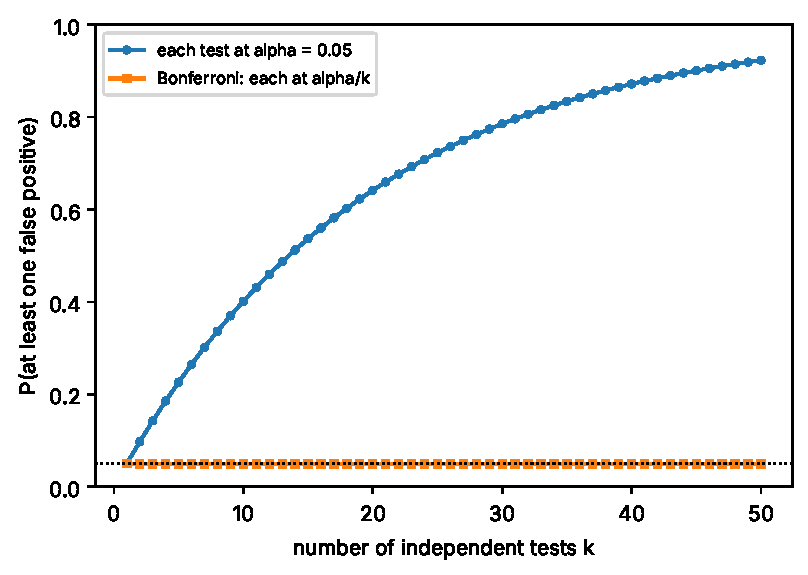
\includegraphics[width=0.85\linewidth]{figs/controls_posthoc.pdf}
\caption{Probability of at least one false positive among $k$ independent tests at level $\alpha=0.05$ (Eq.~\eqref{eq:controls-fwer}), and with the Bonferroni threshold $\alpha/k$. The dotted line marks $0.05$.}\label{fig:controls-posthoc}
\end{figure}

\subsection{Statistics defined after the data were seen}

A subtler version: the statistic itself is invented after looking. Suppose you notice that the frequencies picked out by a sparse fit of the zeros all sit near logarithms of prime powers (Chapter~\ref{ch:sparse-frequency}), and you then design a score for ``how prime-like'' a set of frequencies is. Your design choices (which matching window, which prime powers, which frequency cutoff, how to combine matches into one number) were all made knowing the result for the real data. Even if every choice was reasonable, there were many reasonable alternatives you did not take, and nobody can compute the probability of the score over the space of analyses you might have done. This is sometimes called the ``garden of forking paths''.

Generating surrogates and running \emph{exactly the same} procedure on each (including any maximization over cutoffs) does correct for the steps that are applied identically to real and surrogate data. It does not correct for the choice of the statistic, made after the real outcome was known. That is why such a check is exploratory: it can show that the real data are far from every surrogate under \emph{this} statistic, but it does not license a p-value.

\begin{beyond}
\textbf{A density we quote.} The next Sample Problem uses the prime number theorem in the form ``near $x$, the primes have density about $1/\log x$ per unit length of $x$'' (Chapter~\ref{ch:primes}). Its proof is beyond this book. Prime powers $p^m$ with $m\ge2$ are far rarer than primes and are neglected in the estimate.
\end{beyond}

\begin{sample}{Why matching windows need a cutoff}
A selected frequency $\omega$ is said to ``match'' if $|\omega-\log q|<\pi/T$ for some prime power $q$, where $T$ is the length of the training window in $t$. Take $T=t_{400}-t_1\approx666$. Estimate the expected number of prime powers $q$ whose $\log q$ falls inside the matching window around (a) $\omega=\log13$, (b) $\omega=8$. Estimate the probability of a chance match in each case.

\textbf{Step 1:} Window width in $\log q$: $2\pi/T=2\pi/666=0.00943$.

\textbf{Step 2:} Density of primes per unit of $\log q$. Near $q$ there are about $\dd q/\log q$ primes in $\dd q$. Since $\dd(\log q)=\dd q/q$, we have $\dd q=q\,\dd(\log q)$, so the count per unit of $\log q$ is $q/\log q=e^\omega/\omega$ at $\omega=\log q$.

\textbf{Step 3 (a):} $e^\omega/\omega=13/2.565=5.07$, expected count $5.07\times0.00943=0.048$.

\textbf{Step 4 (b):} $e^8/8=2981/8=372.6$, expected count $372.6\times0.00943=3.5$.

\textbf{Step 5:} Treating the $\log q$ as scattered like a Poisson process at this density (a heuristic; Chapter~\ref{ch:probability} gives the probability of no point in an interval with expected count $\lambda$ as $e^{-\lambda}$), the chance-match probability is $1-e^{-\lambda}$: (a) $1-e^{-0.048}=0.047$; (b) $1-e^{-3.52}=0.970$.

\[
\boxed{\text{(a) }\approx0.05\text{ expected},\ P\approx0.05;\qquad\text{(b) }\approx3.5\text{ expected},\ P\approx0.97}
\]
Near $\omega=8$ almost any frequency matches some prime power by accident, so an alignment statistic needs a frequency cutoff, and \emph{where} the cutoff goes strongly affects the score. A cutoff chosen to maximize the score after seeing the data is a post hoc choice of exactly the kind this section warns about.
\end{sample}

\begin{pitfall}
Do not report an exploratory statistic with a p-value or the word ``significant''. Report what was done, say that the statistic was defined after the data were seen, and if possible confirm on fresh data (here: a new range of zeros never looked at) with the statistic frozen in advance.
\end{pitfall}

\begin{checkpoint}
If you apply the same cutoff maximization to every surrogate as to the real data, which part of the post hoc problem have you fixed, and which remains?
\end{checkpoint}
\checkanswer{Fixed: the inflation from choosing the best cutoff, since surrogates get the same advantage. Remaining: the choice of the statistic itself (matching rule, prime-power range, scoring formula), which was made after seeing the real result.}

\begin{keyideas}
\item Confirmatory: everything fixed in advance; p-values meaningful. Exploratory: data-steered; descriptive only.
\item $k$ independent looks at level $\alpha$ give false-alarm probability $1-(1-\alpha)^k$; Bonferroni uses $\alpha/k$.
\item A statistic designed after seeing the data cannot support a significance claim, even with surrogates.
\end{keyideas}

%======================================================================
\section{Ensembles, seeds, ranges and standard errors}\label{sec:controls-ensembles}

\subsection{Sources of variability}

A computational result can change because of: (1) the data (which zeros were used); (2) the train/test split (which zeros were held out, when chosen at random); (3) the optimizer (random starting coefficients); (4) the surrogate draw. Each source is probed by repeating the computation with different \textbf{seeds} of the random number generator, producing an \textbf{ensemble of replicates}.

Three different summaries of an ensemble of $R$ replicate values $v_1,\dots,v_R$ are common, and they answer different questions:
\begin{itemize}
\item the \textbf{range} $[\min v,\max v]$: ``how different can the result look?'';
\item the \textbf{standard deviation} $s_v$: ``how spread out are individual replicates?'';
\item the \textbf{standard error of the ensemble mean} $s_v/\sqrt R$: ``how precisely is the average known?''; valid only if the replicates are independent draws from the variability one cares about.
\end{itemize}

\subsection{When replicates are not independent samples}

If ten seeds randomly split the \emph{same} 400 zeros into training and test sets, the ten results share the same underlying data. Their spread shows how sensitive the result is to the split, but it says nothing about how the result would change with different zeros. Dividing their standard deviation by $\sqrt{10}$ would give a misleadingly small number. That is why the paper's Table~III caption says: ``The seeds reuse the same zeros, so the ranges indicate robustness and are not standard errors.''

\subsection{From a range to a spread}

For $R$ independent draws from a Gaussian distribution with standard deviation $\sigma$, the expected range is $d_R\sigma$, where $d_R$ is a tabulated constant from quality-control practice: $d_2=1.128$, $d_4=2.059$, $d_{10}=3.078$. It can be written as $d_R=\int_{-\infty}^{\infty}\big[1-\Phi(x)^R-(1-\Phi(x))^R\big]\dd x$, with $\Phi$ the standard Gaussian cumulative distribution. The box below explains where this formula comes from, and the check script evaluates it numerically. So a range over ten seeds is roughly three standard deviations wide, and a range over four repeats about two.

\begin{beyond}
\textbf{Where the formula for $d_R$ comes from.} Let $Z_1,\dots,Z_R$ be independent standard Gaussians.
\begin{itemize}
\item The maximum is $\le x$ exactly when every $Z_i\le x$, so by independence $P(\max\le x)=\Phi(x)^R$.
\item The minimum is $>x$ exactly when every $Z_i>x$, so $P(\min>x)=(1-\Phi(x))^R$.
\end{itemize}
We take on trust the identity $E[Z]=\int_0^\infty P(Z>z)\,\dd z-\int_{-\infty}^0P(Z\le z)\,\dd z$, valid for any random variable with a finite mean. It follows from integration by parts; see \cite{rhb}. Apply it to the maximum and to the minimum, and subtract.
\begin{itemize}
\item On $(0,\infty)$ the integrands combine to $[1-\Phi^R]-(1-\Phi)^R$.
\item On $(-\infty,0)$ they combine to $-\Phi^R+[1-(1-\Phi)^R]$, which is the same expression.
\end{itemize}
So $E[\max-\min]=\int_{-\infty}^{\infty}[1-\Phi(x)^R-(1-\Phi(x))^R]\,\dd x=d_R$. For a Gaussian with standard deviation $\sigma$ every value scales by $\sigma$, so the expected range is $d_R\sigma$.
\end{beyond}

\begin{sample}{Optimizer spread versus sampling uncertainty}
Table~I's caption reports that four random-initialization repeats of the scale-1, $M=400$, zeros 1--400 fit give held-out rms from $0.365$ to $0.379$. Sec.~III gives the bootstrap $95\%$ interval $[0.33,0.43]$ for the held-out rms of a random-restart replicate of this configuration. (The deterministic run from $c=0$, rms $0.369$, has the similar interval $[0.32,0.42]$ in Table~II.) Both intervals are $0.10$ wide. Compare the two sources of variability.

\textbf{Step 1:} Range of the four repeats: $0.379-0.365=0.014$. Estimated standard deviation: $0.014/d_4=0.014/2.059=0.0068$.

\textbf{Step 2:} A $95\%$ interval spans about $\pm1.96$ standard errors if the bootstrap distribution is near-Gaussian, so the held-out sampling SE is about $0.10/3.92=0.0255$.

\textbf{Step 3:} Ratio: $0.0255/0.0068=3.75$.

\[
\boxed{\text{sampling SE}\approx0.026,\ \text{optimizer spread}\approx0.007,\ \text{ratio}\approx3.8}
\]
Which held-out levels were scored matters several times more than where the optimizer started. Both are small next to the gap between $0.369$ and the null $0.263$. (These are rough conversions, valid for near-Gaussian spreads; they are meant only for comparing orders of magnitude.)
\end{sample}

\subsection{Good reporting practice}

\begin{itemize}
\item State what was varied (seed for split, for initialization, for surrogate), how many replicates, and how they were summarized.
\item Use ``mean $\pm$ SD over $R$ draws'' or a range when replicates share data; reserve standard errors for independent samples.
\item Report seeds, so anyone can regenerate the ensemble exactly.
\item When a result depends on an analysis choice (block length, ridge strength, a threshold), report a range of choices and say whether conclusions change.
\item Record changes made after a first attempt (for instance, ``added once, after a first version was unstable, and not tuned'').
\end{itemize}

\begin{checkpoint}
Ten surrogate draws give in-sample rms with mean $0.134$ and spread $0.010$. Is $0.010$ an uncertainty on the mean $0.134$?
\end{checkpoint}
\checkanswer{Not directly; it describes how much individual surrogate fits differ. If the ten draws are independent and $0.010$ is their standard deviation, the uncertainty of the mean is about $0.010/\sqrt{10}=0.003$.}

\begin{keyideas}
\item Range, SD and SE of an ensemble answer different questions; replicates sharing the same data give robustness ranges, not standard errors.
\item For $R$ Gaussian draws the expected range is $d_R\sigma$ ($d_4=2.059$, $d_{10}=3.078$).
\item Report seeds and the sensitivity of conclusions to analysis choices.
\end{keyideas}

%======================================================================
\section{Paper connection}\label{sec:controls-paper}

The paper \cite{soniR1} uses every tool of this chapter. Table~\ref{tab:controls-paper} maps them; we then go through each use.

\begin{table}[htbp]\centering
\caption{Where the tools of this chapter appear in the paper (R1 numbering).}\label{tab:controls-paper}
\begin{tabular}{ll}
\toprule
tool & paper location\\
\midrule
independent bootstrap, percentile 95\% & Sec.~III; Tables II, IV, V captions; App.~A steps 13, 22\\
circular / moving block bootstrap & Sec.~III (``Other bases''); App.~A step 22\\
permutation surrogate & Sec.~III; App.~A steps 12, 18\\
phase-randomized and IAAFT surrogates & Sec.~III; App.~A step 18; refs.~\cite{theiler,schreiber}\\
surrogate ensembles for an alignment check & Sec.~IV; App.~A step 23\\
positive controls & Sec.~III (continuation probe); Sec.~II D (oracle)\\
leakage controls & Sec.~II C (Eq.~(3)); App.~A step 20\\
seeds, ranges vs.\ standard errors & Tables I and III captions; App.~A step 17\\
exploratory qualification & Sec.~IV; App.~A step 23\\
proposed standard & Sec.~VI, items (i)--(iv)\\
\bottomrule
\end{tabular}
\end{table}

\paragraph{Bootstrap intervals for operator fits (Sec.~III, Table~II).} Appendix~A step 13 records the recipe: ``$2\times10^4$ resamples of held-out indices; percentile 95\% intervals for rms and correlation'', exactly the Monte Carlo percentile bootstrap of Sec.~\ref{sec:controls-bootstrap}, with prediction--truth pairs resampled together. Sec.~III reports, for the scale-1, $M=400$ random-restart replicate, OOS rms $[0.33,0.43]$ against the null $0.263$, and correlation $[-0.21,+0.08]$; for scale 2, $M=600$, rms $[0.26,0.30]$ against null $0.274$ and correlation $[-0.18,+0.08]$. The paper describes the first as ``significantly worse than the null'' and the second as ``consistent with its null''. In the language of this chapter: the first interval lies entirely above the null value; the second contains it. Both correlation intervals contain zero. On the same 401--500 holdout, the six-prime oracle's correlation interval is $[+0.95,+0.97]$, which you reproduced in the fourth Sample Problem.

Table~II attaches intervals to every alternative-basis row. Note the Chebyshev $M=400$ row, $0.291$ $[0.25,0.33]$ and $+0.18$ $[-0.02,+0.37]$: the rms interval contains the null $0.263$, and the correlation interval's lower end is at (slightly below) zero. The paper reports this honestly as ``marginal'': ``one such row among eight is not evidence of prediction, but a small positive correlation for this row is not excluded.'' This is the multiple-looks issue of Sec.~\ref{sec:controls-posthoc} in the other direction: among eight rows, one marginal row is roughly what chance alone produces.

\paragraph{Serial correlation and the block bootstrap (Sec.~III, App.~A step 22).} The Table~II caption warns: the intervals ``resample held-out levels independently although the fluctuations are serially correlated''. Sec.~III continues: ``recomputed with a moving-block bootstrap (block lengths 3 to 20) they widen slightly and no conclusion changes (for the cosine row, at most $[0.30,0.44]$)''; step 22 specifies a circular block bootstrap on zeros 401--500. This is the sensitivity-over-$\ell$ procedure of Sec.~\ref{sec:controls-block}. The Discussion (Sec.~VI) restates the limitation: ``Bootstrap intervals resample held-out levels independently except where stated.''

\paragraph{Intervals for the arithmetic models (Sec.~IV, Tables IV and V).} The Table~IV caption gives intervals on 401--500: A (900 terms) $[0.015,0.020]$, B (900) $[0.158,0.201]$, C1 $[0.231,0.285]$, C2 $[0.028,0.041]$, against null $0.263$. Sec.~IV adds C1's correlation interval $[+0.08,+0.46]$. Reading them: the A, B and C2 intervals lie far below the null; the C1 rms interval contains the null, so ``capacity without a suitable prior does not generalize'', even though its correlation interval sits above zero. The Table~V caption gives the six-prime oracle's correlation intervals $[+0.95,+0.97]$ (401--500) and $[+0.91,+0.92]$ (5001--10000); the second is narrower because it uses 5000 held-out levels instead of 100, as the $1/\sqrt n$ law of Sec.~\ref{sec:controls-variability} leads you to expect.

\paragraph{Surrogate refits: structure or capacity (Sec.~III; App.~A steps 12, 18).} Step 18 defines the surrogates on the fluctuation sequence in mean spacings, $d_n=(\tilde t_n-E_n[\text{smooth}])/\gap_n$ for $n\le400$ (here $\tilde t_n$ are the bias-corrected targets and $E_n[\text{smooth}]$ the levels of the unperturbed Wu--Sprung potential): ``permutation; phase randomization (real FFT, uniform phases); IAAFT (200 iterations); seeds 1--10; targets $E_n[\text{smooth}]+d'_n\gap_n$, refit with $M=400$''. Your \texttt{phase\_randomize} and \texttt{iaaft} functions implement the same recipes. The results (the Sample Problem ``Reading the paper's surrogate refits'' in Sec.~\ref{sec:controls-capacity}) show the operator family fits all three surrogates as well as the true zeros. Sec.~III also explains a change from the original submission: permuting fluctuations in energy units ``also moves amplitude across heights'' and gave $0.148$, $0.149$ (step 12 anchors $0.1483/0.1493$ for seeds 1 and 2); permuting in spacing units keeps the amplitude at each height, which is ``the cleaner control''. Choosing which properties a surrogate keeps is the core design decision of Sec.~\ref{sec:controls-surrogates}.

\paragraph{Held-out surrogates and the kriging positive control (Sec.~III; App.~A steps 18, 19).} The paper does not stop at in-sample refits. A linear interpolator (simple kriging, Chapter~\ref{ch:generalization}) ``predicts held-out true zeros at $0.117$ with correlation $+0.87$ and permuted targets at the null'', which is a positive control: it shows the serial structure of the zeros is real and usable, and the permuted negative control confirms the interpolator is not exploiting anything else. The fitted operator, held out the same way, ``fails alike on true zeros and on surrogates ($0.57$--$0.70$; one split, illustrative)''. Note the honest qualifiers: one split, illustrative. Step 19 also records a forking path transparently: ``projection and nugget were added once, after a first version without them was numerically unstable, and not tuned.''

\paragraph{Positive controls with known answers (Secs.~II D, III).} The arithmetic-continuation probe of Sec.~III replaces the targets by the pure prime-2 oscillation (running example RE2; Appendix~A step 15). The right continuation is known exactly; the family ``represents it almost perfectly in-sample (rms $0.056$, correlation $+0.95$) and continues it not at all (held-out correlation $+0.07$, rms worse than predicting zero fluctuation)''. The oracle (Sec.~II D) plays the complementary role: it is ``an information-existence baseline'' showing that predictable structure exists. A negative result (``the operator does not predict'') is only informative when such positive controls show that prediction is possible.

\paragraph{Leakage controls (Sec.~II C, App.~A step 20).} Two controls guard against held-out data influencing the fit. One is algebraic: Eq.~(3) shows that scoring against bias-corrected targets equals correcting the prediction by a fit-independent quantity $\Delta_n$ built from unperturbed eigenvalues only. The other is empirical, in step 20: ``Overwriting held-out data with noise before fitting leaves all fitted coefficients bit-identical.'' This is the leakage control of Sec.~\ref{sec:controls-capacity} in its cleanest form.

\paragraph{The surrogate alignment check, and why it is exploratory (Sec.~IV; App.~A step 23).} The sparse sinusoidal control C2 selects frequencies from the zeros, and every one lies near some $\log p^m$. Because ``the frequencies are the output of a search'', the paper reruns ``the complete procedure on surrogate zero sets: phase-randomized surrogates and two families of sparse signals with non-arithmetic frequencies, 900 replicates in all''. Step 23 gives the composition: 200 (fit 1--400) and 100 (fit 1--800) replicates of each of three families, $3\times(200+100)=900$, with match criterion $|\omega-\log q|<\pi/T$, $q\le3000$, and a ``cutoff-maximized binomial score $24.7$ and $50.9$ on the real zeros, at most $4.7$ on surrogates (score defined after the data were seen)''. The paper's own words are measured: ``the qualifications that apply (the statistic was defined after the data were seen, so the check is exploratory) are documented in the reconstruction record \cite{zenodo}; no significance claim is made here beyond the size of the ensembles.'' After Sec.~\ref{sec:controls-permutation} you can unpack the last phrase: with no surrogate reaching the real score, an ensemble of 200 could at most support $p\le1/201\approx0.005$, and one of 100 at most $p\le1/101\approx0.01$; and because the score was designed post hoc (Sec.~\ref{sec:controls-posthoc}), even those bounds are not offered as p-values. The paper refers to the reconstruction record for the construction of the surrogates and of the score; this book does not reproduce them. Note also, from the chance-match Sample Problem, why a frequency cutoff is needed at all: near $\omega=8$ a window of width $2\pi/T$ catches a prime power by chance with probability close to 1. Finally, the paper stresses that the underlying fact, that the Fourier transform of the zeros concentrates at logarithms of prime powers, is classical \cite{landau,gonek}; the check concerns only whether the search procedure recovers it.

\paragraph{Seeds and ensembles (Tables I and III captions; App.~A step 17).} Table~I's caption reports ``four random-init repeats \ldots\ give identical in-sample rms $0.1370$ and OOS $0.365$--$0.379$'' and ``three repeats of the (scale~2, $M=600$) row give OOS $0.279$--$0.283$'': ranges, summarizing optimizer variability, which the last Sample Problem showed to be several times smaller than held-out sampling uncertainty. The within-height random splits use ``\texttt{rng.choice(n, n/5, replace=False)}, seeds 1--10'' (step 17), and Table~III reports ranges over seeds with the explicit caveat that they ``are not standard errors''.

\paragraph{The proposed standard (Sec.~VI).} The paper proposes that any claim that an operator ``captures'' the zeros come with: (i) a train/test split, including one within a height range; (ii) scoring of the actual operator spectrum; (iii) ``evidence that performance survives regularization and restarts'' (an ensemble over seeds and settings, Sec.~\ref{sec:controls-ensembles}); and (iv) ``a refit to permuted and phase-randomized targets'' (negative controls, Sec.~\ref{sec:controls-capacity}). Two of the four items are exactly this chapter's subject.

\paragraph{Rerunning at small scale.} With \texttt{qmnt}, the null rms on zeros 401--500 (smooth zeros as prediction) is $0.2631$, matching the paper's anchor (Appendix~A, ``null OOS (401--500) $0.2631$''), and the six-prime oracle and its bootstrap interval are reproduced by the listing in Sec.~\ref{sec:controls-bootstrap}. The surrogate and operator refits require \texttt{qmnt.fit\_potential} and take minutes per fit; Problems~22 and 32 ask for related small-scale computations that do not need \texttt{fit\_potential}.

%======================================================================
\section{Summary}

\begin{itemize}
\item Every score is a draw from a sampling distribution; for iid data the SE of a mean is $\sigma/\sqrt n$ (Eq.~\eqref{eq:controls-varmean}), estimated by $s/\sqrt n$ (Eq.~\eqref{eq:controls-se}).
\item The bootstrap resamples the data with replacement; for the mean its exact variance is $\hat\sigma^2/n$ (Eq.~\eqref{eq:controls-bootvarmean}); there are $\binom{2n-1}{n}$ distinct resamples (Eq.~\eqref{eq:controls-distinct}); percentile intervals take quantiles of the replicates.
\item For a stationary sequence, $\mathrm{Var}(\bar X)=(\gamma_0/n)f_n$ with $f_n=1+2\sum_k(1-k/n)\rho_k$ (Eq.~\eqref{eq:controls-varcorr}); AR(1) gives $\rho_k=\varphi^k$ and $f_\infty=(1+\varphi)/(1-\varphi)$ (Eq.~\eqref{eq:controls-finf}).
\item The circular block bootstrap keeps dependence within blocks of length $\ell$; for the mean its variance is Eq.~\eqref{eq:controls-cbbvar}. Report results over a range of $\ell$.
\item Permutation tests test exchangeability; Monte Carlo p-values are $(1+r)/(N+1)$ (Eq.~\eqref{eq:controls-mcp}), bounded below by $1/(N+1)$.
\item Surrogates: permutation keeps the marginal; phase randomization keeps spectrum and circular autocorrelation (Eq.~\eqref{eq:controls-wk}); IAAFT keeps the marginal exactly and the spectrum approximately (Table~\ref{tab:controls-surr}).
\item Negative, positive and leakage controls decide whether a fit reflects structure or capacity; a family that fits surrogates as well as real data shows capacity only.
\item $k$ looks at level $\alpha$ give $1-(1-\alpha)^k$ false-alarm probability (Eq.~\eqref{eq:controls-fwer}); statistics defined after seeing the data are exploratory.
\item Ranges over seeds that reuse the same data indicate robustness, not standard errors; for $R$ Gaussian draws the expected range is $d_R\sigma$.
\end{itemize}

%======================================================================
\section{Problems}

\begin{problemlist}
\prob{1}{Data $(2,5,8)$. Compute $\bar x$, $s$, $\widehat{\mathrm{SE}}(\bar x)=s/\sqrt n$ and the ideal bootstrap SE $\sqrt{\hat\sigma^2/n}$.}
\prob{1}{How many distinct bootstrap resamples (as multisets) exist for $n=4$ data points? How many ordered resamples?}
\prob{1}{Which of the three surrogate families of Table~\ref{tab:controls-surr} would you use to keep (a) exactly the same set of values, (b) exactly the same power spectrum, (c) both, as nearly as possible?}
\prob{1}{In a Monte Carlo test, 3 of 99 surrogates have a statistic at least as large as the real one. What is the p-value?}
\prob{2}{Enumerate the bootstrap distribution of the mean for the data $(0,1)$ ($n=2$). Compute its variance and check Eq.~\eqref{eq:controls-bootvarmean}.}
\prob{2}{For an AR(1) sequence with $\varphi=0.8$, find the large-$n$ inflation factor $f_\infty$ and the effective sample size of $n=1000$ observations. Interpret.}
\prob{2}{Evaluate $f_{200}$ for $\varphi=-0.5$ using Eq.~\eqref{eq:controls-fn}, and the corresponding effective sample size.}
\prob{2}{A mean-zero sequence $x_1,\dots,x_n$ is randomly permuted. Show that the expected value of the lag-1 product $x_{\pi(i)}x_{\pi(i+1)}$ is $\big[(\sum_jx_j)^2-\sum_jx_j^2\big]/[n(n-1)]=-\sum_jx_j^2/[n(n-1)]$, so the expected normalized lag-1 autocorrelation is about $-1/(n-1)$. Evaluate it for $n=400$.}
\prob{2}{Show that phase randomization preserves the mean and the sum of squares $\sum_jd_j^2$ of a real sequence. (Use $D_0$ and Parseval's theorem for the DFT, $\sum_jd_j^2=\frac1n\sum_q|D_q|^2$.)}
\prob{2}{For $n=20$ and $\ell=4$, how many moving blocks are there? How many blocks contain observations 1, 2 and 10? How many circular blocks are there, and how many contain each observation?}
\prob{2}{Using Table~II of the paper, list the rows whose bootstrap rms interval excludes the null $0.263$, and those whose correlation interval excludes zero. What do the latter say?}
\prob{2}{Using the Table~IV caption intervals of the paper, decide for each of A (900 terms), B (900), C1 and C2 whether the rms interval lies below, contains, or lies above the null $0.263$.}
\prob{2}{Appendix~A of the paper anchors the original-submission permutation test (energy units) at in-sample rms $0.1483$ and $0.1493$ (seeds 1 and 2), against $0.1370$ on true targets. By what percentages are these worse? Explain, using the fact that the mean spacing $\gap_n$ decreases with $n$, why permuting in energy units changes the amplitude profile in spacing units.}
\prob{1}{With $k=10$ independent looks at $\alpha=0.05$, what is the probability of at least one false positive?}
\prob{2}{None of $N=200$ surrogates reaches the real statistic. (a) Give the Monte Carlo p-value. (b) Find the largest exceedance probability $q$ consistent, at $95\%$ confidence, with seeing zero exceedances, by solving $(1-q)^{200}=0.05$, and compare with the ``rule of three'' $3/N$.}
\prob{2}{Table~III of the paper reports random-split in-sample rms $0.20$--$0.22$ over ten seeds (scale 1, $M=200$). Estimate the seed-to-seed standard deviation using $d_{10}$, and explain why you would not divide it by $\sqrt{10}$.}
\prob{2}{Sec.~IV of the paper says ``no significance claim is made here beyond the size of the ensembles''. For each fit range in Appendix~A step 23, what is the smallest Monte Carlo p-value that a single surrogate family could support if no replicate reached the real score?}
\prob{3}{Derive Eq.~\eqref{eq:controls-varcorr} for a stationary sequence, then derive Eq.~\eqref{eq:controls-fn} for AR(1) without neglecting the tail, i.e.\ find $\sum_{k=1}^{n-1}(1-k/n)\varphi^k$ exactly.}
\prob{3}{Using numpy, simulate AR(1) sequences with $\varphi=0.5$, $n=400$ and unit noise variance. For block lengths $\ell=1,5,20$ compute the average circular-block-bootstrap SE of the mean over many series and compare with the true SE from Eq.~\eqref{eq:controls-varcorr} and the prediction of Eq.~\eqref{eq:controls-cbbvar} with the true autocovariances.}
\prob{2}{Using numpy, phase-randomize $d=(1,2,0,-1)$ with $\phi=\pi/2$ and with $\phi=\pi$ applied to $D_1$. Show that both surrogates are circular shifts of $d$, and explain why a sequence with a single nonzero non-real Fourier pair can only produce shifted (or interpolated-shift) surrogates.}
\prob{2}{Using qmnt, compute the null rms (smooth zeros as prediction) on zeros 401--500, and the six-prime oracle's rms and correlation there. Compare with Table~V of the paper.}
\prob{3}{Using qmnt and numpy, compute circular-block-bootstrap $95\%$ intervals for the six-prime oracle's correlation on zeros 401--500, for $\ell=3,5,10,20$, and compare with the independent bootstrap. Does any conclusion change?}
\prob{3}{Using numpy, generate an IAAFT surrogate of the RE2 target (Fig.~\ref{fig:controls-surrogates}) with 200 iterations. Verify that its sorted values equal the original's exactly and compute the relative rms difference between its Fourier magnitudes and the original's. How does that difference evolve with the number of iterations?}
\prob{2}{Explain how a \emph{paired} bootstrap would compare a model's held-out rms with the null's: what is resampled, what statistic is computed on each resample, and why this is preferable to comparing the model's interval with a fixed null value.}
\prob{2}{The paper's alignment check (Sec.~IV; App.~A step 23) runs the full sparse-frequency search on 900 surrogates and computes a ``cutoff-maximized'' score on each. Which part of the post hoc problem does this design handle, and which remains? Why does the paper call the check exploratory?}
\prob{1}{Ten independent surrogate draws have in-sample rms standard deviation $0.010$. What is the standard error of their mean?}
\prob{3}{Prove that for two groups of equal size $m$, the exact permutation distribution of the difference of means $D=\bar x_A-\bar x_B$ is symmetric about zero, whatever the data.}
\prob{2}{In the paper's within-height analysis (Sec.~III), the six-prime oracle scores $0.062$--$0.063$ on the same held-out sets where operator fits score above the null. Which role (positive or negative control, or neither) does the oracle play there, and why is it needed to interpret the operator's failure?}
\prob{3}{Repeat the chance-match estimate of Sec.~\ref{sec:controls-posthoc} at $\omega=\log101$ with $T=666$. What does the result suggest about the frequency range in which an alignment with prime-power logarithms is informative?}
\prob{2}{The kriging interpolator of the paper predicts held-out true zeros with correlation $+0.87$ and permuted targets at the null (Sec.~III). Explain which part of this is a positive control and which a negative control, and what each establishes.}
\prob{2}{With $B=2\times10^4$ Monte Carlo bootstrap replicates, which sorted positions give the $2.5\%$ and $97.5\%$ percentile endpoints? Roughly how accurate is the bootstrap SE as an estimate of the ideal bootstrap SE?}
\prob{3}{Using numpy, reproduce Fig.~\ref{fig:controls-capacity}. Then replace the six-function structured model by one with the wrong frequencies (say $m\log3$, $m=1,2,3$) and show that it fits neither the real target nor the surrogates well. What does this say about using surrogate refits with a misspecified model?}
\end{problemlist}

%======================================================================
\section{Answers to selected problems}

\begin{enumerate}
\item[1.] $\bar x=5$; deviations $-3,0,3$, squares sum $18$; $s^2=18/2=9$, $s=3$; $\widehat{\mathrm{SE}}=3/\sqrt3=1.732$. Plug-in $\hat\sigma^2=18/3=6$, ideal bootstrap variance $6/3=2$, SE $=\sqrt2=1.414$ (ratio $\sqrt{2/3}$, as Eq.~\eqref{eq:controls-bootvarmean} predicts).
\item[2.] Eq.~\eqref{eq:controls-distinct}: $\binom74=35$ multisets; ordered resamples $4^4=256$.
\item[3.] (a) Permutation (or IAAFT). (b) Phase randomization. (c) IAAFT: exact marginal, approximate spectrum. No standard method gives both exactly.
\item[4.] $r=3$, $N=99$: $p=(1+3)/(99+1)=0.04$.
\item[5.] Ordered resamples $(0,0),(0,1),(1,0),(1,1)$, means $0,\tfrac12,\tfrac12,1$ with probabilities $\tfrac14,\tfrac12,\tfrac14$. Mean $\tfrac12$; $E[\bar x^{*2}]=\tfrac14\cdot0+\tfrac12\cdot\tfrac14+\tfrac14\cdot1=\tfrac38$; variance $\tfrac38-\tfrac14=\tfrac18$. Formula: $\hat\sigma^2=\tfrac12[(\tfrac12)^2+(\tfrac12)^2]=\tfrac14$, divided by $n=2$: $\tfrac18$. Agreement.
\item[7.] $\varphi/(1-\varphi)=-1/3$, $\varphi/(1-\varphi)^2=-0.2222$; $f_{200}=1+2[-0.33333+0.2222/200]=0.3356$; $n_{\rm eff}=200/0.3356=596$.
\item[9.] The mean is $D_0/n$ and $\phi_0=0$, so $D_0$ is unchanged. Each $|D_q|$ is unchanged, so by Parseval $\sum_jd_j'^2=\frac1n\sum_q|D_q'|^2=\frac1n\sum_q|D_q|^2=\sum_jd_j^2$. Mean and sum of squares fixed imply the variance is fixed.
\item[11.] rms interval excludes $0.263$ (all lie above it): cosine 400 $[0.32,0.42]$; Chebyshev 200 $[0.32,0.42]$; Chebyshev 600 $[0.64,0.82]$; hat 200 $[0.30,0.38]$; hat 400 $[0.29,0.39]$; hat 600 $[0.29,0.37]$. Six rows. The Chebyshev 400 $[0.25,0.33]$ and Chebyshev $\mu=0.3$ $[0.24,0.29]$ intervals contain the null. Only hat 400 has a correlation interval excluding zero, $[-0.37,-0.01]$, and it is \emph{negative}: anticorrelation with the truth, consistent with the fit-induced damage discussed in the paper, not with skill.
\item[13.] $0.1483/0.1370=1.082$ and $0.1493/0.1370=1.090$: about $8\%$ and $9\%$ worse. In energy units a fluctuation is $d_n\gap_n$. Low-$n$ levels have large $\gap_n$, so their energy-unit fluctuations are large; permuting moves some of them to high $n$, where dividing by the smaller $\gap_n$ makes them large in spacing units, and moves small ones to low $n$. The surrogate's amplitude in spacings then varies with height, unlike the real one, so the control changes more than the serial order.
\item[14.] $1-0.95^{10}=1-0.5987=0.4013$.
\item[15.] (a) $p=1/201=0.004975$. (b) $\ln(1-q)=\ln(0.05)/200=-0.014979$, so $q=1-e^{-0.014979}=0.01487$; the rule of three gives $3/200=0.015$, nearly the same because $-\ln0.05=2.996\approx3$ and $\ln(1-q)\approx-q$ for small $q$.
\item[17.] Each family has 200 replicates for the 1--400 fit and 100 for the 1--800 fit (Appendix~A step 23). If no replicate reaches the real score, Eq.~\eqref{eq:controls-mcp} gives at most $p=1/201\approx0.005$ and $p=1/101\approx0.010$, respectively. And because the score was defined after the data were seen, the paper does not offer even these as p-values.
\item[19.] True SE: $\gamma_0=1/(1-0.25)=4/3$, $f_{400}=1+2(1-2/400)=2.99$, SE $=\sqrt{(4/3)(2.99)/400}=0.0998$. Independent bootstrap ($\ell=1$): about $\sqrt{(4/3)/400}=0.0577$. Eq.~\eqref{eq:controls-cbbvar} with true autocovariances: $\ell=5$: $1+2(0.8\cdot0.5+0.6\cdot0.25+0.4\cdot0.125+0.2\cdot0.0625)=2.225$, SE $0.0861$; $\ell=20$: factor $2.8$, SE $0.0966$. Your simulated averages should sit close to these, slightly lower because the sample mean is estimated (Fig.~\ref{fig:controls-ar1}, right).
\item[21.] Null rms $0.2631$, matching the paper's anchor and the $0.263$ entry of Table~V; six-prime oracle rms $0.074$ and correlation $+0.96$, matching Table~V's ``6 primes'' column, row 401--500.
\item[23.] The sorted values agree exactly because the last step of each iteration is the rank-order remap, which places the original values in the new order. The relative magnitude mismatch falls quickly during the first iterations and then levels off at a small value (the paper reports spectra matched ``to 1\%'' for its surrogates, Sec.~III); it cannot reach zero in general, because an exact marginal and an exact spectrum are not simultaneously attainable for generic data.
\item[25.] Running the same search and the same cutoff maximization on every surrogate gives the surrogates the same opportunity to look aligned, which accounts for the search over frequencies and the choice of cutoff. What remains is the choice of the statistic itself (matching criterion, prime-power range, binomial scoring), designed after the real result was known; its distribution over the analyses one might have chosen is unknown. Hence ``exploratory'', and ``no significance claim \ldots\ beyond the size of the ensembles''.
\item[26.] If the ten draws are independent and $0.010$ is their standard deviation, SE $=0.010/\sqrt{10}=0.0032$.
\item[27.] Every relabeling chooses a set $A$ of $m$ positions; its complement $B$ also has $m$ positions. The map ``swap $A$ and $B$'' is a one-to-one correspondence of the set of $\binom{2m}{m}$ relabelings onto itself, and it sends $D=\bar x_A-\bar x_B$ to $-D$. So for every value $D$ the number of relabelings giving $D$ equals the number giving $-D$, and the distribution is symmetric about zero.
\item[29.] $e^\omega/\omega=101/4.615=21.9$; times $2\pi/666=0.00943$ gives about $0.21$ expected prime powers in the window, so a chance match has probability roughly $1-e^{-0.21}\approx0.19$. Already at $q\approx100$ one frequency in five would match by accident, against about one in twenty near $q=13$ and almost all near $q=3000$: alignment carries most of its information at low frequencies, and the statistic must weigh matches by how unlikely they are by chance.
\item[31.] Positions $\lceil0.025\times20000\rceil=500$ and $\lceil0.975\times20000\rceil=19500$. For a near-Gaussian bootstrap distribution the relative error of the SE estimate is about $1/\sqrt{2B}=1/200=0.5\%$.
\end{enumerate}
